% !TeX program = lualatex
\documentclass[10pt,letterpaper,oneside,openany]{report}

\usepackage[letterpaper,top=0.78in,bottom=0.84in,left=0.82in,right=0.82in,headheight=15pt]{geometry}
\usepackage{amsmath,mathtools}
\usepackage{fontspec}
\usepackage{unicode-math}
\defaultfontfeatures{Ligatures=TeX,Scale=MatchLowercase}
\setmainfont{LibertinusSerif}[
  Extension=.otf,
  UprightFont=*-Regular,
  ItalicFont=*-Italic,
  BoldFont=*-Bold,
  BoldItalicFont=*-BoldItalic
]
\setsansfont{LibertinusSans}[
  Extension=.otf,
  UprightFont=*-Regular,
  ItalicFont=*-Italic,
  BoldFont=*-Bold
]
\setmonofont{DejaVu Sans Mono}[Scale=0.82]
\setmathfont{LibertinusMath-Regular.otf}

\usepackage{microtype}
\usepackage{xcolor}
\usepackage{booktabs,tabularx,longtable,array,multirow}
\usepackage{enumitem}
\usepackage{fvextra}
\usepackage[most]{tcolorbox}
\usepackage{tikz}
\usetikzlibrary{arrows.meta,positioning,fit,calc,shapes.geometric,backgrounds}
\usepackage{titlesec}
\usepackage{fancyhdr}
\usepackage{needspace}
\usepackage[bottom]{footmisc}
\usepackage{xurl}
\usepackage{hyperref}
\usepackage{bookmark}

\definecolor{Ink}{HTML}{24302D}
\definecolor{MutedInk}{HTML}{56635F}
\definecolor{Paper}{HTML}{F8F5ED}
\definecolor{Panel}{HTML}{EFF3EE}
\definecolor{PanelBlue}{HTML}{EEF3F7}
\definecolor{PanelGold}{HTML}{F8F1E4}
\definecolor{PanelRed}{HTML}{F8ECEA}
\definecolor{Sage}{HTML}{4F705F}
\definecolor{SageDark}{HTML}{315142}
\definecolor{Blue}{HTML}{2B5E7E}
\definecolor{Gold}{HTML}{A66A18}
\definecolor{Red}{HTML}{943E3E}
\definecolor{Rule}{HTML}{C9D1CB}
\definecolor{CodeBack}{HTML}{F1F4F0}

\pagecolor{white}
\color{Ink}
\hypersetup{
  colorlinks=true,
  linkcolor=SageDark,
  citecolor=Blue,
  urlcolor=Blue,
  pdfauthor={OpenAI},
  pdftitle={Lean from First Principles: Dependent Types, the Calculus of Constructions, and Leant},
  pdfsubject={A beginner introduction to Lean sufficient to understand Leant and Djex},
  pdfkeywords={Lean 4, dependent types, calculus of constructions, CIC, Leant, Djex, program synthesis}
}
\urlstyle{same}

\setlength{\parindent}{0pt}
\setlength{\parskip}{0.55em}
\setlength{\emergencystretch}{3em}
\raggedbottom
\setlist[itemize]{leftmargin=1.45em,itemsep=0.22em,topsep=0.25em}
\setlist[enumerate]{leftmargin=1.65em,itemsep=0.22em,topsep=0.25em}
\setlist[description]{style=nextline,leftmargin=1.8em,labelsep=0.45em,itemsep=0.35em}

\titleformat{\chapter}[display]
  {\normalfont\sffamily\bfseries\color{SageDark}}
  {\filleft\Large\color{Sage}\chaptername\ \thechapter}
  {0.35ex}
  {\titlerule[0.7pt]\vspace{0.8ex}\Huge\raggedright\hyphenpenalty=10000\exhyphenpenalty=10000\relax}
\titlespacing*{\chapter}{0pt}{-12pt}{24pt}
\titleformat{\section}{\Large\sffamily\bfseries\color{SageDark}}{\thesection}{0.7em}{}
\titleformat{\subsection}{\large\sffamily\bfseries\color{Blue}}{\thesubsection}{0.65em}{}
\titleformat{\subsubsection}{\normalsize\sffamily\bfseries\color{Ink}}{\thesubsubsection}{0.6em}{}

\pagestyle{fancy}
\fancyhf{}
\fancyhead[L]{\small\sffamily\color{MutedInk}\nouppercase{\leftmark}}
\fancyhead[R]{\small\sffamily\color{MutedInk}Lean from First Principles}
\fancyfoot[C]{\small\sffamily\color{MutedInk}\thepage}
\renewcommand{\headrulewidth}{0.35pt}
\renewcommand{\footrulewidth}{0pt}
\fancypagestyle{plain}{
  \fancyhf{}
  \fancyfoot[C]{\small\sffamily\color{MutedInk}\thepage}
  \renewcommand{\headrulewidth}{0pt}
}

\tcbset{
  enhanced,
  breakable,
  boxrule=0.6pt,
  arc=1.5mm,
  left=2.6mm,right=2.6mm,top=2.0mm,bottom=2.0mm,
  before skip=0.7em,after skip=0.8em,
  fonttitle=\sffamily\bfseries,
  coltitle=white
}
\newtcolorbox{keyidea}[1][Key idea]{colback=Panel,colframe=SageDark,colbacktitle=SageDark,title={#1}}
\newtcolorbox{firstlook}[1][First look]{colback=PanelBlue,colframe=Blue,colbacktitle=Blue,title={#1}}
\newtcolorbox{implementation}[1][Implementation note]{colback=PanelBlue,colframe=Blue,colbacktitle=Blue,title={#1}}
\newtcolorbox{leantbox}[1][Why this matters for Leant]{colback=PanelGold,colframe=Gold,colbacktitle=Gold,title={#1}}
\newtcolorbox{warningbox}[1][Boundary]{colback=PanelRed,colframe=Red,colbacktitle=Red,title={#1}}
\newtcolorbox{sourcebox}[1][Source trail]{colback=white,colframe=Rule,colbacktitle=MutedInk,title={#1}}
\newtcolorbox{recapbox}[1][Chapter checkpoint]{colback=Paper,colframe=Sage,colbacktitle=Sage,title={#1}}
\newtcolorbox{formalbox}[1][Formal rule]{colback=white,colframe=Blue,colbacktitle=Blue,title={#1}}

\newcommand{\CodeTitle}{Lean}
\newenvironment{leanblock}[1][Lean]
  {\def\CodeTitle{#1}\VerbatimEnvironment\begin{VerbatimOut}{\jobname-code.tmp}}
  {\end{VerbatimOut}
   \begin{tcolorbox}[colback=CodeBack,colframe=Rule,colbacktitle=SageDark,title={\CodeTitle},
     sharp corners=south,breakable=false]
   \VerbatimInput[fontsize=\small,breaklines=true,breakanywhere=true,tabsize=2]{\jobname-code.tmp}
   \end{tcolorbox}}

\newcommand{\term}[1]{\texttt{\detokenize{#1}}}
\newcommand{\kw}[1]{\textsf{\textbf{#1}}}
\newcommand{\LeantCommit}{\texttt{49c8f9f100a6}}
\newcommand{\DjexCommit}{\texttt{0cf82f2aa22d}}
\newcommand{\DjexPinnedCommit}{\texttt{7d65eba6f753}}
\newcommand{\LeanCommit}{\texttt{79c4cd09fdab}}
\newcommand{\PiTy}[3]{\Pi (#1 : #2),\,#3}
\newcommand{\defeq}{\mathrel{\equiv}}
\newcommand{\judges}[3]{#1\;\vdash\;#2 : #3}
\newcommand{\blankline}{\par\vspace{0.25em}}

\begin{document}
\hypersetup{pageanchor=false}

\begin{titlepage}
\centering
\vspace*{0.7in}
{\sffamily\bfseries\color{SageDark}\fontsize{34}{40}\selectfont
Lean from First Principles\par}
\vspace{0.35in}
{\sffamily\color{Blue}\fontsize{19}{24}\selectfont
Dependent Types, the Calculus of Constructions,\par
and the Architecture of Leant\par}
\vspace{0.55in}
{\large A beginner's path from ``a term has a type'' to verified type-directed synthesis}
\vfill
\begin{tcolorbox}[width=0.84\textwidth,colback=Paper,colframe=Sage,colbacktitle=SageDark,
  title=Repository snapshot]
\small
\begin{tabularx}{\linewidth}{@{}>{\bfseries}l X@{}}
Leant & \LeantCommit\ (main, inspected 16 August 2026)\\
Djex used by Leant & \DjexPinnedCommit\ (the \texttt{lib/Djex} submodule)\\
Djex standalone & \DjexCommit\ (main, inspected for the current shared architecture)\\
Lean 4 & \LeanCommit\ (master)\\
\end{tabularx}
\end{tcolorbox}
\vfill
{\sffamily\color{MutedInk}Prepared 16 August 2026}
\end{titlepage}

\pagenumbering{roman}

\chapter*{Preface}
\addcontentsline{toc}{chapter}{Preface}

This guide has a deliberately narrow destination and a deliberately broad runway.  The destination is practical: after reading it, an absolute beginner should be able to open the Leant and Djex repositories, understand what problem \term{:synth} is trying to solve, follow the major data transformations, and judge correctly what a successful candidate or a negative result means.  The runway is broad because those facts make little sense until Lean's central idea is internalized: \emph{types may depend on values, propositions are types, and proofs are ordinary typed terms checked by a small kernel}.

The guide is not a general catalogue of Lean tactics, a mathlib tutorial, or a replacement for the official Lean books.  It concentrates on the pieces that determine Leant's design:

\begin{itemize}
\item the Curry--Howard correspondence and type inhabitation;
\item dependent function types, dependent pairs, universes, inductive families, equality, and transport;
\item the Calculus of Constructions and the inductive extension used by Lean;
\item the separation between surface syntax, elaboration, metaprogramming, and kernel expressions;
\item the gap between Lean's rich dependent type theory and Djex's deliberately smaller Haskell-like synthesis language;
\item the translation, search, rendering, verification, and evidence boundaries in Leant.
\end{itemize}

The existing LaTeX documents in the Leant repository use two useful idioms.  The user manual in \path{docs/Leant.tex} uses LuaLaTeX and Unicode-safe transcript boxes; the longer architecture reports use chapters, pinned revisions, source trails, diagrams, and explicit trust-boundary boxes.  This document combines those idioms.  All Lean snippets are presented as Unicode-capable verbatim material, and source-specific statements are tied to the pinned repository state above.

\begin{keyidea}[The one-sentence thesis]
Lean provides the rich language and the final type checker; Leant projects selected Lean goals into a smaller synthesis problem for Djex, turns Djex's answers back into Lean syntax, and asks Lean to accept or reject every displayed candidate.
\end{keyidea}

\section*{How to read this guide}

For the shortest route to the Leant implementation, read Chapters~\ref{ch:first-lean}--\ref{ch:inhabitation}, then Chapters~\ref{ch:pi}--\ref{ch:equality}, and finally Parts~\ref{part:implementation} and~\ref{part:leant}.  The formal-rule boxes can be skipped on a first pass.  They are there to remove ambiguity when one later reads kernel code or reasons about completeness.

A few notational conventions recur:

\begin{itemize}
\item $\Gamma \vdash t : A$ means that in context $\Gamma$, term $t$ has type $A$.
\item $A \to B$ is a non-dependent function type.
\item $\Pi (x : A), B(x)$ is a dependent function type; Lean writes it as \term{(x : A) → B x} or \term{∀ x : A, B x}.
\item $t \defeq u$ means \emph{definitionally equal}: Lean can see the equality by computation and built-in conversion rules, without an explicit equality proof.
\item ``kernel'' always means the trusted checker for fully elaborated terms, not the parser, elaborator, tactic engine, or synthesis engine.
\end{itemize}

\tableofcontents
\clearpage
\pagenumbering{arabic}
\hypersetup{pageanchor=true}

\part{The Core Idea}

\chapter{A First Encounter with Lean}\label{ch:first-lean}

\section{Lean is both a language and a checker}

Lean is a functional programming language, a language for stating mathematical propositions, and an interactive theorem prover.  These are not three unrelated subsystems bolted together.  They share one typed term language.  A natural number expression is a term.  A function is a term.  A proposition is a type.  A proof is a term whose type is that proposition.

Start with ordinary programming:

\begin{leanblock}[Lean: data and functions]
def twice (f : Nat → Nat) (x : Nat) : Nat :=
  f (f x)

#check twice
#eval twice (fun n => n + 1) 40
\end{leanblock}

The declaration says that \term{twice} accepts a function from natural numbers to natural numbers, accepts a natural number, and returns a natural number.  The body is checked against that declared type.  Evaluation produces \term{42}.

Now look at a theorem written in the same language:

\begin{leanblock}[Lean: a proof as a function]
theorem andSwap (P Q : Prop) : P ∧ Q → Q ∧ P :=
  fun h => ⟨h.right, h.left⟩
\end{leanblock}

The body is again a term checked against a type.  This time the type is a proposition.  The input \term{h} contains proofs of both $P$ and $Q$; the output pair puts them in the opposite order.  Nothing in the kernel says ``switch into proof mode now.''  It checks one typed term.

\begin{firstlook}[Read the punctuation literally]
In \term{P ∧ Q → Q ∧ P}, the arrow is right-associative, so the type means ``given a proof of $P \land Q$, produce a proof of $Q \land P$.''  The term \term{fun h => ...} is a lambda expression: a function accepting that proof.
\end{firstlook}

\section{Declarations: \texttt{def}, \texttt{theorem}, \texttt{example}, and \texttt{opaque}}

The most common top-level forms differ mainly in how the result is named and how it may compute.

\begin{description}
\item[\term{def}] Introduces a named definition with a body.  Lean may unfold it during computation and definitional equality, subject to transparency policy in higher layers.
\item[\term{theorem}] Introduces a named proof.  Its body is checked, but theorem bodies are treated opaquely by kernel reduction after acceptance.  This keeps proof checking manageable and expresses that the proof's type is the public contract.
\item[\term{example}] Checks a declaration without adding a durable user-facing name.  It is ideal for experiments and, notably, for Leant's candidate-verification command.
\item[\term{opaque}] Introduces a checked constant whose implementation does not unfold during ordinary reduction.  It is useful when only a signature should be visible.
\item[\term{axiom}] Introduces a constant with a stated type and no body.  The kernel checks later reasoning relative to that assumption; it does not prove the axiom.
\end{description}

Leant verifies a rendered candidate by asking Lean to elaborate a noncomputable example of exactly the requested type:

\begin{leanblock}[The shape of Leant's verification command]
set_option autoImplicit true in
noncomputable example : (GOAL) := (CANDIDATE)
\end{leanblock}

That small command is architecturally decisive.  The candidate is not accepted because Djex says it has the right type, nor because a string renderer believes it is valid.  Lean elaborates it in the live environment and the kernel checks the resulting expression.

\section{Terms, types, and types of types}

Lean's \texttt{\#check} command asks the elaborator to report a term's type:

\begin{leanblock}[Lean: inspecting types]
#check 17
#check Nat
#check Nat → Nat
#check fun x : Nat => x + 1
#check Prop
#check Type
#check Type 1
\end{leanblock}

Typical results are conceptually:

\begin{center}
\begin{tabular}{@{}ll@{}}
\toprule
Term & Type \\
\midrule
\term{17} & \term{Nat} \\
\term{Nat} & \term{Type} \\
\term{Nat → Nat} & \term{Type} \\
\term{fun x : Nat => x + 1} & \term{Nat → Nat} \\
\term{Prop} & \term{Type} \\
\term{Type} & \term{Type 1} \\
\term{Type 1} & \term{Type 2} \\
\bottomrule
\end{tabular}
\end{center}

A type is itself a term, classified by a universe.  This is the first hint of the Calculus of Constructions: the language does not stop at functions between data values.  It can quantify over types, compute types, and form functions whose results are types.

\section{What Leant adds}

Lean already has holes, tactics, simplifiers, type-class search, decision procedures, and powerful proof automation.  Leant adds a particular interactive workflow inspired by GHCi and Djinn:

\begin{leanblock}[A representative Leant interaction]
:synth ((A → B → C) → (A → B) → A → C)
\end{leanblock}

A natural answer is:

\begin{leanblock}[Synthesized Lean term]
fun f g x => f x (g x)
\end{leanblock}

The type determines a wiring diagram.  Given $f : A \to B \to C$, $g : A \to B$, and $x : A$, the only direct way to build $C$ is to give $f$ an $A$ and a $B$; $x$ supplies the first, and $g\,x$ supplies the second.

Leant's job is not merely to print a plausible lambda term.  It must:

\begin{enumerate}
\item ask Lean to elaborate the requested goal into a precise internal expression;
\item decide which structure can be translated into a synthesis fragment and which must remain opaque;
\item run one or both Djex engines under explicit search policies;
\item reconstruct Lean syntax, including binders, constructors, global names, and implicit arguments erased by the search model;
\item re-elaborate each candidate against the exact original goal;
\item report negative results only with the strength justified by both translation completeness and search completeness.
\end{enumerate}

\begin{leantbox}
The beginner's temptation is to think of Leant as ``Lean plus a clever autocomplete.''  A more accurate model is a verified compiler pipeline with a lossy middle language.  Candidate soundness comes from checking the trip back into Lean; negative evidence depends on proving that the lossy projection was not lossy for this particular query.
\end{leantbox}

\begin{sourcebox}
The current Leant overview and examples are in \url{https://github.com/VladimirReshetnikov/Leant/blob/49c8f9f100a644b5a32b3c942bc6565a3a3ba6a0/README.md}.  The exact candidate command is generated by \path{src/Leant/Synth/Fragment.hs}; process management is in \path{src/Leant/Backend.hs}; orchestration and interactive state are in \path{src/Main.hs}.
\end{sourcebox}

\begin{recapbox}
You should now be able to read ``a proof of $P$'' as ``a term of type $P$,'' and ``synthesize a program of type $T$'' as ``search for an inhabitant of $T$.''  Lean owns the exact type theory and final check.  Leant owns an interactive translation/search/reconstruction pipeline around that checker.
\end{recapbox}

\chapter{Reading Lean Syntax Without Fear}\label{ch:syntax}

Lean's notation is dense because the same core constructs serve programming and proof.  This chapter decodes the subset needed throughout the guide and in the Leant source.

\section{Function types and function values}

A function type is written with an arrow:

\begin{leanblock}[Function signatures]
Nat → Nat
String → Nat → Bool
(A → B) → A → B
\end{leanblock}

Arrows associate to the right:

\[
A \to B \to C \quad\text{means}\quad A \to (B \to C).
\]

Function application is written by juxtaposition and associates to the left:

\[
f\;x\;y \quad\text{means}\quad (f\;x)\;y.
\]

A lambda expression introduces arguments:

\begin{leanblock}[Equivalent lambda spellings]
fun x : Nat => x + 1
fun (x : Nat) => x + 1
fun x y => x + y
\end{leanblock}

Multiple arguments are syntactic convenience for nested one-argument functions.  This is \emph{currying}:

\[
\lambda x.\lambda y.\,t
\]

has type $A \to B \to C$ when $x:A$, $y:B$, and $t:C$.

\section{Named parameters and binder styles}

Lean has four binder styles that matter both to users and to Leant's renderer:

\begin{center}
\begin{tabularx}{\textwidth}{@{}l l X@{}}
\toprule
Surface form & Binder information & Normal use \\
\midrule
\term{(x : A)} & explicit & caller supplies an ordinary argument \\
\term{{x : A}} & implicit & elaborator usually infers the argument \\
\term{{{x : A}}} & strict implicit & inferred only once a later explicit argument is present \\
\term{[x : C]} & instance implicit & type-class synthesis supplies evidence \\
\bottomrule
\end{tabularx}
\end{center}

For example:

\begin{leanblock}[Implicit and instance arguments]
def ident {α : Sort u} (x : α) : α := x

class Named (α : Type u) where
  name : α → String

def display {α : Type u} [Named α] (x : α) : String :=
  Named.name x
\end{leanblock}

The braces around $\alpha$ say that Lean should infer the type from \term{x}.  The square brackets say that Lean should search the current local and global instance environment for a \term{Named α} value.

\begin{leantbox}[Why binder visibility survives translation]
Djinn's logical model does not natively distinguish every Lean binder visibility.  Leant therefore records whether a quantified type binder was explicit, implicit, or instance-implicit, and its renderer may insert lambdas or \term{_} placeholders that the search term itself never contained.  A single semantic candidate can consequently produce several textual variants, only one of which elaborates.
\end{leantbox}

\section{Definitions by equations and pattern matching}

Lean lets functions be written as pattern-matching equations:

\begin{leanblock}[Structural recursion on lists]
def append : List α → List α → List α
  | [], ys => ys
  | x :: xs, ys => x :: append xs ys
\end{leanblock}

This notation is elaborated into recursors and auxiliary definitions.  The kernel does not trust the equation compiler; it checks the generated term.

Constructor patterns expose the data carried by an inductive value:

\begin{leanblock}[Pattern matching on a sum]
def either (f : A → C) (g : B → C) : A ⊕ B → C
  | .inl a => f a
  | .inr b => g b
\end{leanblock}

A \term{match} expression gives the same structure inline:

\begin{leanblock}[Inline match]
fun s : A ⊕ B =>
  match s with
  | .inl a => Sum.inr a
  | .inr b => Sum.inl b
\end{leanblock}

\section{Products, structures, and constructor notation}

The type \term{A × B} is an ordinary product.  A value can be written \term{(a, b)} or, when the expected type identifies a one-constructor structure, with anonymous constructor brackets \term{⟨a, b⟩}.  Fields can be projected by names or indices.

\begin{leanblock}[Products and projections]
def swap (p : A × B) : B × A :=
  ⟨p.2, p.1⟩
\end{leanblock}

The same anonymous constructor notation works for conjunction because \term{And} is a proposition-valued inductive type with one constructor:

\begin{leanblock}[The same shape in Prop]
theorem andSwap' (P Q : Prop) : P ∧ Q → Q ∧ P :=
  fun h => ⟨h.2, h.1⟩
\end{leanblock}

Leant exploits expected-type elaboration here.  Its renderer can use universe-agnostic shapes such as \term{⟨a, b⟩}, and Lean decides whether the target is \term{Prod}, \term{And}, \term{PProd}, or another compatible structure.

\section{Unicode and ASCII}

Lean's standard notation uses symbols such as \term{→}, \term{∀}, \term{∧}, \term{∨}, \term{¬}, \term{⟨}, and \term{⟩}.  Editors insert them through abbreviations; ASCII alternatives exist for many constructs.  The important point is semantic, not typographic:

\begin{center}
\begin{tabular}{@{}lll@{}}
\toprule
Lean & Read as & Core idea \\
\midrule
\term{A → B} & function / implication & non-dependent $\Pi$ \\
\term{∀ x : A, P x} & for every $x$ & dependent $\Pi$ \\
\term{P ∧ Q} & conjunction & product-like inductive in \term{Prop} \\
\term{P ∨ Q} & disjunction & sum-like inductive in \term{Prop} \\
\term{¬ P} & not $P$ & definitionally $P \to \mathsf{False}$ \\
\term{∃ x, P x} & there exists $x$ & inductive existential in \term{Prop} \\
\bottomrule
\end{tabular}
\end{center}

\section{Term mode and tactic mode}

A theorem body can be a direct term:

\begin{leanblock}[Direct proof term]
theorem compose (f : B → C) (g : A → B) : A → C :=
  fun x => f (g x)
\end{leanblock}

or a tactic script beginning with \term{by}:

\begin{leanblock}[Tactic proof producing the same kind of term]
theorem compose' (f : B → C) (g : A → B) : A → C := by
  intro x
  exact f (g x)
\end{leanblock}

Tactics manipulate goals and construct a term behind the scenes.  The kernel receives only the final elaborated term.  Leant's \term{:prove} mode participates at the goal-manipulation layer, while \term{:synth} chiefly asks for a whole inhabitant of a target type.

\begin{recapbox}
Arrows and applications have opposite associativity; binders carry visibility information; pattern matching is compiled; products and conjunctions can share constructor-shaped syntax; tactic scripts are programs that build proof terms.  These facts explain many seemingly fussy steps in Leant's renderer.
\end{recapbox}

\chapter{Propositions Are Types, Proofs Are Terms}\label{ch:curry-howard}

\section{The Curry--Howard dictionary}

The correspondence used by Lean can be summarized as follows:

\begin{center}
\begin{tabularx}{0.94\textwidth}{@{}X X@{}}
\toprule
Logic & Type theory \\
\midrule
proposition $P$ & type $P : \mathsf{Prop}$ \\
proof of $P$ & term $p : P$ \\
$P \Rightarrow Q$ & function type $P \to Q$ \\
$P \land Q$ & type with a proof of $P$ and a proof of $Q$ \\
$P \lor Q$ & type tagged with either a proof of $P$ or a proof of $Q$ \\
$\top$ & inhabited unit-like proposition \\
$\bot$ & empty proposition \\
$\forall x:A,\,P(x)$ & dependent function returning a proof for every $x$ \\
$\exists x:A,\,P(x)$ & package containing a witness and a proof \\
proof normalization & program reduction \\
\bottomrule
\end{tabularx}
\end{center}

This is not merely an analogy used in documentation.  The kernel type checks proofs using the same mechanisms used to type check functions.

\section{Implication is a function}

To prove $P \to Q$, assume a proof of $P$ and construct a proof of $Q$:

\begin{leanblock}[Implication introduction]
theorem idProof (P : Prop) : P → P :=
  fun p => p
\end{leanblock}

To use a proof of $P \to Q$, apply it to a proof of $P$:

\begin{leanblock}[Implication elimination]
theorem modusPonens (P Q : Prop) : (P → Q) → P → Q :=
  fun hpq hp => hpq hp
\end{leanblock}

The words ``introduction'' and ``elimination'' name the two directions of constructor use.  Introduction builds a value of a type; elimination consumes one.  Djinn's LJT proof search is largely a disciplined automation of these structural moves.

\section{Conjunction is product-like}

To prove $P \land Q$, provide both components.  To use it, project or pattern-match:

\begin{leanblock}[Conjunction]
theorem reassoc (P Q R : Prop) :
    (P ∧ Q) ∧ R → P ∧ (Q ∧ R) :=
  fun h => ⟨h.1.1, ⟨h.1.2, h.2⟩⟩
\end{leanblock}

The exact type \term{And P Q} lives in \term{Prop}; \term{Prod P Q} would live in a data universe if $P$ and $Q$ were data types.  Their logical shapes are similar, but Lean keeps the nominal families distinct.

\section{Disjunction is sum-like}

A proof of $P \lor Q$ contains a tag saying which side holds.  Introduction chooses a tag; elimination handles both cases:

\begin{leanblock}[Disjunction]
theorem orSwap (P Q : Prop) : P ∨ Q → Q ∨ P :=
  fun h =>
    match h with
    | Or.inl hp => Or.inr hp
    | Or.inr hq => Or.inl hq
\end{leanblock}

This is the same computational shape as swapping \term{Sum A B}, though proof irrelevance changes what may later be observed from proposition-valued data.

\section{Truth, falsity, and negation}

\term{True} has a constructor, so it is inhabited.  \term{False} has no constructors, so a proof of it cannot be built in a consistent context.  But if a hypothesis already has type \term{False}, it can be eliminated into any proposition or type:

\begin{leanblock}[Explosion]
theorem absurdFromFalse (P : Prop) : False → P :=
  fun h => False.elim h
\end{leanblock}

Negation is defined as implication to falsity:

\[
\neg P \quad\text{is}\quad P \to \mathsf{False}.
\]

So a proof of \term{¬ P} is a function that turns any hypothetical proof of $P$ into contradiction.

\section{Universal and existential quantification}

A universal proof is a dependent function:

\begin{leanblock}[Universal quantification]
theorem eqSelf : ∀ n : Nat, n = n :=
  fun n => Eq.refl n
\end{leanblock}

An existential proof packages a witness and evidence:

\begin{leanblock}[Existential witness]
theorem existsEven : ∃ n : Nat, n % 2 = 0 :=
  ⟨0, rfl⟩
\end{leanblock}

The witness can affect the type of the second component.  That dependency is why quantifiers are not reducible to ordinary simple function and pair types.

\section{Constructive logic and classical additions}

The core proof interpretation is constructive: a proof should carry enough information to construct its conclusion.  For example, a proof of $P \lor Q$ identifies a side.  The law of excluded middle, $P \lor \neg P$, is not derivable for an arbitrary proposition from constructive rules alone.

Lean's libraries can add classical principles through named axioms and derived theorems.  Once such a constant is in the term, the kernel can check the term relative to it.  The distinction matters in Leant:

\begin{itemize}
\item Djinn's LJT engine searches intuitionistic logic.
\item Leant can optionally offer classical premises after a constructive route is exhausted or refuted.
\item A candidate using classical principles is still type-correct Lean, but its axiom dependencies differ.
\end{itemize}

Lean can report the assumptions on which a declaration depends with \texttt{\#print axioms name}.

\begin{warningbox}[Type correctness is relative to the environment]
The kernel proves no theorem ``from reality.''  It checks that a term has a type using the declarations and axioms in its environment.  Sound engineering therefore tracks not only whether a term checks, but which opaque constants, axioms, instance declarations, and imported definitions it relies on.
\end{warningbox}

\begin{recapbox}
Logical connectives have data-like introduction and elimination rules.  This turns proof search into typed term synthesis.  Djinn can automate a propositional structural fragment because that fragment has a finite, well-understood proof calculus; Lean's full dependent language is richer and requires additional care.
\end{recapbox}

\chapter{Type Inhabitation Is Program Synthesis}\label{ch:inhabitation}

\section{The question asked by a type}

Given a type $T$, the inhabitation problem asks:

\begin{quote}
Does there exist a term $t$ such that $t : T$?  If so, construct one.
\end{quote}

For a proposition, this is theorem proving.  For a data type, it is program construction.  For a mixed dependent type, it can be both at once.

Some types have an obvious canonical inhabitant:

\begin{leanblock}[Canonical inhabitants]
fun x : A => x

fun f : A → B => fun g : B → C => fun x : A => g (f x)

fun p : A × B => (p.2, p.1)
\end{leanblock}

Other types are uninhabited without additional assumptions:

\begin{leanblock}[A structurally impossible polymorphic function]
∀ A B : Type, A → B
\end{leanblock}

After the caller chooses $A$, $B$, and a value of $A$, no source of a $B$ is available.  In a total, parametric language, no term can manufacture an arbitrary value of an arbitrary type.

\section{A type constrains wiring, not behavior completely}

A type can determine a surprising amount of structure.  The type

\[
(A \to B \to C) \to (A \to B) \to A \to C
\]

essentially forces composition.  But many types admit several behaviors:

\begin{leanblock}[Many inhabitants, different behavior]
Nat → Nat

List α → List α

Bool → Bool
\end{leanblock}

For \term{List α → List α}, possible total inhabitants include identity, reverse, constant empty, duplicate each element, drop every element, and many more.  Type-directed synthesis alone cannot know which behavior the user intended.

This gives two distinct kinds of specification:

\begin{description}
\item[Structural specification] Which inputs, outputs, polymorphic variables, sums, products, and constraints must fit together.  This is what Djinn and Exference principally exploit.
\item[Behavioral specification] Equations, invariants, refinement predicates, resource bounds, or examples that distinguish extensionally different inhabitants of the same type.
\end{description}

Current Leant is strongest on structural synthesis.  Its optional Length layer is a deliberately narrow example of behavioral assessment: after ordinary Lean type verification, certain list-spine candidates can be interpreted under a sealed length contract and checked through bounded, replayed arithmetic reasoning.

\section{Soundness and completeness are different promises}

Suppose a tool prints a candidate.  Candidate \emph{soundness} asks whether the printed term really has the requested Lean type.  Leant answers this by re-elaboration and kernel checking.

Suppose instead the tool prints ``uninhabited.''  That is a \emph{completeness} claim about the search and translation.  To justify it, the tool must know that:

\begin{itemize}
\item every relevant part of the Lean goal was represented faithfully;
\item every allowed premise and constructor was included;
\item no hidden type-class dictionary or opaque constant could carry useful data;
\item the search procedure was complete for the represented logic;
\item no configured budget, depth bound, queue pruning, or finite instantiation plan left unexplored cases.
\end{itemize}

A verifier can easily reject a bad positive candidate.  It cannot rescue an unjustified negative claim, because there is no candidate to check.

\begin{keyidea}[The asymmetry that shapes Leant]
A lossy translation can still produce sound positive answers if every answer is checked in the original language.  The same lossy translation cannot support a sound ``no answer exists'' conclusion unless the loss is proven irrelevant for that query.
\end{keyidea}

\section{Search as proof construction}

For the propositional fragment, the type's outer constructor suggests the next proof step:

\begin{center}
\begin{tabularx}{\textwidth}{@{}l X X@{}}
\toprule
Goal shape & Introduction move & Resulting work \\
\midrule
$A \to B$ & introduce $x:A$ & synthesize $B$ in extended context \\
$A \land B$ & build a pair & synthesize both $A$ and $B$ \\
$A \lor B$ & choose an injection & synthesize one branch \\
$\top$ & use unit constructor & done \\
$\bot$ & no introduction rule & must derive from context \\
atomic $P$ & use a hypothesis or premise & apply something whose result is $P$ \\
\bottomrule
\end{tabularx}
\end{center}

Left rules explain how hypotheses can be consumed.  For a hypothesis $h:A\land B$, split it.  For $h:A\lor B$, case-analyze both branches.  For $h:A\to B$, synthesize an $A$ and apply $h$ to obtain $B$.  A focused or contraction-free calculus controls the order so proof search terminates and avoids redundant duplication.

This is the logical heart of Djinn.  Exference reaches similar terms by a different, heuristic best-first exploration over typed expression states.

\begin{sourcebox}
Djinn's object language and proof terms are defined in \url{https://github.com/VladimirReshetnikov/Djex/blob/0cf82f2aa22debb1de2c7aaa13a2abbe190550d8/djinn/src-core/Djinn/Internal/LJTFormula.hs}.  The contraction-free LJT search and its explicit completeness/budget distinction are in \path{djinn/src-core/Djinn/Internal/LJT.hs}.  Exference's priority-queue-driven engine is in \path{exference/src-core/Language/Haskell/Exference/Core/Internal/Exference.hs}.
\end{sourcebox}

\begin{recapbox}
Inhabitation unifies theorem proving and program synthesis.  Types strongly constrain structure but often underdetermine behavior.  Positive soundness can be recovered by checking candidates in Lean; negative completeness requires an exact fragment and exhaustive search.
\end{recapbox}

\part{Dependent Type Theory}

\chapter{Judgments, Contexts, and Substitution}\label{ch:judgments}

Dependent type theory is easiest to understand as a small collection of judgments and rules.  The notation may look formal, but it merely makes explicit what Lean's elaborator and kernel are tracking.

\section{The typing judgment}

The central judgment is

\[
\judges{\Gamma}{t}{A},
\]

read ``under assumptions $\Gamma$, term $t$ has type $A$.''  The context is an ordered list of declarations such as

\[
\Gamma = (A : \mathsf{Type},\; B : \mathsf{Type},\; f : A \to B,\; x : A).
\]

From this context we can derive $\Gamma \vdash f\,x : B$.

Order matters because later types may mention earlier variables.  This context is valid:

\[
(A : \mathsf{Type},\; x : A,\; P : A \to \mathsf{Prop},\; h : P\,x).
\]

The type of $x$ mentions $A$; the type of $P$ mentions $A$; the type of $h$ mentions both $P$ and $x$.  Reordering the entries arbitrarily would make names appear before their declarations.

\section{Variable and weakening rules}

If a context contains $x:A$, then $x$ may be used at type $A$:

\begin{formalbox}[Variable]
\[
\frac{}{\Gamma, x:A, \Delta \vdash x:A}
\]
provided the context is well formed.
\end{formalbox}

A derivation that does not use a new assumption remains valid after that assumption is added.  This is weakening.  In code, adding a local variable does not invalidate earlier expressions, though dependent references require the context to remain ordered.

\section{Substitution is the engine of dependency}

Suppose a body has a free variable $x$:

\[
\Gamma, x:A \vdash t : B(x).
\]

If another term $a$ has type $A$, substitution replaces $x$ by $a$ everywhere:

\[
\Gamma \vdash t[a/x] : B(a).
\]

The crucial point is that substitution occurs not only in the term but also in its type.  This is what distinguishes dependent application from ordinary function application.

In Lean, if

\begin{leanblock}[A dependent function]
f : (n : Nat) → Vector α n
k : Nat
\end{leanblock}

then \term{f k} has type \term{Vector α k}.  The argument $k$ is substituted into the codomain.

\section{Binding, alpha-equivalence, and capture avoidance}

The terms

\[
\lambda x:A.\,x
\qquad\text{and}\qquad
\lambda y:A.\,y
\]

mean the same thing.  Bound variable names are presentation aids; renaming them consistently does not change the term.  This is alpha-equivalence.

A substitution implementation must avoid accidentally capturing free variables.  If one substitutes $y$ for $x$ in $\lambda y.\,x$, naively obtaining $\lambda y.\,y$, the formerly free $y$ has been captured.  The binder must first be renamed, for example:

\[
(\lambda z.\,x)[y/x] = \lambda z.\,y.
\]

Lean's kernel representation avoids many name-management problems by using de Bruijn indices for bound variables.  Djex's shared source types and proof terms instead carry explicit identities and therefore contain binder freshening, alpha-normalization, rigid/flexible variable distinctions, and capture-avoiding substitution machinery.

\begin{implementation}[Locally nameless Lean expressions]
A kernel lambda body represents its bound variable with \term{Expr.bvar 0}; an outer binder is \term{bvar 1}, and so on.  During traversals, Lean commonly instantiates bound variables with fresh free-variable identifiers in a local context.  The names printed to users do not determine binding identity.
\end{implementation}

\section{Metavariables are temporary unknowns}

During elaboration, Lean may know that a term must exist before it knows the term.  It represents such holes with metavariables.  A metavariable has a local context and an expected type; tactics and unification assign it later.

For example, elaborating

\begin{leanblock}[An inferred argument]
List.nil
\end{leanblock}

creates an unknown element type $\alpha$ until the surrounding expected type or later constraints determine it.  Similarly, the placeholder \term{_} asks the elaborator to create and solve a metavariable.

Metavariables are not accepted by the kernel.  The source definition of \term{Lean.Expr} explicitly permits \term{mvar} because the same expression datatype is used by the elaborator, but the kernel type checker rejects any expression that still contains one.

\begin{leantbox}
Leant's serializer runs inside Lean's metaprogramming layer, where it can instantiate metavariables, weak-head normalize expressions, inspect binder information, ask whether a term is a class application, and query inductive declarations.  Its output must describe a closed enough fragment for Haskell to consume.  Later, rendered candidates deliberately reintroduce \term{_} only as surface syntax so Lean can perform a fresh, exact elaboration.
\end{leantbox}

\begin{recapbox}
A typing judgment is always relative to an ordered context.  Dependency means substitution changes types as well as terms.  Bound names are not identities.  Metavariables are elaboration-time obligations, never kernel-level proof holes.
\end{recapbox}

\chapter{Dependent Function Types: The Pi-Type}\label{ch:pi}

\section{From arrows to dependent arrows}

An ordinary function type $A \to B$ says that every input has the same result type $B$.  A dependent function type permits the result type to mention the input:

\[
\Pi (x:A),\,B(x).
\]

Lean uses several surface forms for this one core construction:

\begin{leanblock}[Pi-type notation]
(x : A) → B x
∀ x : A, B x
{x : A} → B x
[x : C] → B x
\end{leanblock}

When $x$ does not occur in $B$, the dependent product degenerates to an ordinary arrow:

\[
A \to B \quad\text{is notation for}\quad \Pi (_:A),\,B.
\]

This is why the kernel needs only one constructor, \term{Expr.forallE}, for both function types and universal quantification.

\section{Formation, introduction, and elimination}

The formation rule says that if $A$ is a type and $B(x)$ is a type for each $x:A$, then the dependent function type is a type:

\begin{formalbox}[$\Pi$ formation]
\[
\frac{
  \Gamma \vdash A : \mathsf{Sort}\;u
  \qquad
  \Gamma,x:A \vdash B : \mathsf{Sort}\;v
}{
  \Gamma \vdash \Pi(x:A),B : \mathsf{Sort}(\operatorname{imax}(u,v))
}
\]
\end{formalbox}

Introduction is lambda abstraction:

\begin{formalbox}[$\Pi$ introduction]
\[
\frac{\Gamma,x:A \vdash t : B}
     {\Gamma \vdash (\lambda x:A.\,t) : \Pi(x:A),B}
\]
\end{formalbox}

Elimination is application, with substitution in the result type:

\begin{formalbox}[$\Pi$ elimination]
\[
\frac{
  \Gamma \vdash f : \Pi(x:A),B(x)
  \qquad
  \Gamma \vdash a : A
}{
  \Gamma \vdash f\,a : B(a)
}
\]
\end{formalbox}

These three rules simultaneously explain ordinary functions, polymorphism, universal quantification, and type constructors.

\section{Four uses of the same constructor}

\subsection{Functions from values to values}

\begin{leanblock}[Ordinary function]
def successor : Nat → Nat := fun n => n + 1
\end{leanblock}

The codomain does not depend on $n$.

\subsection{Functions from types to values}

\begin{leanblock}[Polymorphic identity]
def ident {α : Sort u} (x : α) : α := x
\end{leanblock}

The function quantifies over a type $\alpha$ and then over a value of that type.  Its full type is approximately

\[
\Pi(\alpha : \mathsf{Sort}\;u),\,\alpha \to \alpha.
\]

\subsection{Functions from values to types}

\term{Vector α} maps a natural number to a type:

\begin{leanblock}[A type family]
#check Vector
-- Vector : Type u → Nat → Type u
\end{leanblock}

For fixed $\alpha$, \term{Vector α 3} and \term{Vector α 4} are different types.  A type family is simply a function whose codomain is a universe.

\subsection{Functions from types to types}

\term{List} is a type constructor:

\begin{leanblock}[A polymorphic type constructor]
#check List
-- List : Type u → Type u
\end{leanblock}

At the kernel level, this is again an ordinary constant whose type is a $\Pi$-type.

\section{Universal propositions are dependent functions}

The proposition

\[
\forall n:\mathbb{N},\; n=n
\]

is represented by a dependent function type whose codomain lies in \term{Prop}.  Its proof is a function returning a proof for each input:

\begin{leanblock}[A universal proof]
theorem reflAll : ∀ n : Nat, n = n :=
  fun n => rfl
\end{leanblock}

The notation \term{∀} changes how humans read the type, not the kernel constructor.

\section{Dependency can be computationally relevant}

Consider a function that returns a vector whose length is its input:

\begin{leanblock}[Result type depends on the argument]
def replicateVec (α : Type u) (a : α) :
    (n : Nat) → Vector α n
  | 0 => Vector.nil
  | n + 1 => Vector.cons a (replicateVec α a n)
\end{leanblock}

For each $n$, the result has a different type.  The recursive branch must return exactly \term{Vector α (n + 1)}, not merely ``some vector.''  The type checker tracks the index through the computation.

This expressive power is precisely what a simply typed search calculus lacks.  Djinn can treat an entire formula such as \term{∀ n, P n} as an opaque atom and move it around, but it cannot generally synthesize a term by inspecting $n$, changing a result index, or transporting across an equality.

\section{Rank and prenex quantification}

A type is rank-1 when universal quantifiers appear only at the outermost level.  A higher-rank type places a polymorphic function inside an argument:

\begin{leanblock}[A rank-2 shape]
((∀ α : Type, α → α) → Nat)
\end{leanblock}

Djex's shared Haskell-like type representation supports explicit \term{ForallType} layers and bounded handling of certain higher-rank uses.  But the quantifier is still a type-scheme mechanism, not full term dependency.  Leant must preserve Lean binder visibility and, for some instantiations, enumerate reconstruction variants.

\begin{keyidea}[Do not confuse two meanings of ``forall'']
In Lean, every function binder is represented by the same dependent $\Pi$ constructor.  In Djex's source type language, \term{ForallType} means Haskell-style type-variable quantification, while \term{FunctionType} means a value-level arrow.  Leant's translation decides how a Lean \term{forallE} maps across that split.
\end{keyidea}

\begin{recapbox}
The $\Pi$-type unifies functions, polymorphism, universal proofs, and type families.  Application substitutes the argument into the result type.  Lean's single kernel constructor is richer than Djex's separate Haskell-style forall and arrow constructors, so translation is semantic rather than syntactic.
\end{recapbox}

\chapter{Dependent Pairs, Subtypes, and Existence}\label{ch:sigma}

\section{The Sigma-Type}

A dependent pair packages a first component $x:A$ and a second component whose type may depend on $x$:

\[
\Sigma(x:A),\,B(x).
\]

Lean's general dependent pair is \term{Sigma}:

\begin{leanblock}[A length-indexed package]
def SomeVector (α : Type u) :=
  Sigma fun n : Nat => Vector α n
\end{leanblock}

A value of \term{SomeVector α} contains a natural number $n$ and a vector of exactly that length.  The second projection's type depends on the first projection.

\begin{leanblock}[Constructing and consuming a Sigma]
def oneVector (a : α) : SomeVector α :=
  ⟨1, Vector.cons a Vector.nil⟩

def packedLength (v : SomeVector α) : Nat :=
  v.1
\end{leanblock}

The ordinary product $A \times B$ is the non-dependent special case where $B$ ignores the first component.

\section{Why dependent pairs are harder to translate}

A structural synthesis engine can represent a pair as ``produce an $A$ and a $B$.''  For a dependent pair it must instead produce an $a:A$ and then produce a term of $B(a)$.  The second search problem is not even known until the first term is chosen.  If $B(a)$ contains computation, equality, or indexed inductives, simple propositional search is insufficient.

Leant therefore expands only carefully characterized product-like inductives with non-dependent fields.  A genuinely dependent structure, such as a constructor whose later field type mentions an earlier field, remains opaque to Djinn's structural logic.

\section{Subtypes}

A subtype packages data together with a proposition about it:

\begin{leanblock}[A bounded natural number]
def SmallNat := {n : Nat // n < 10}

def three : SmallNat :=
  ⟨3, by decide⟩
\end{leanblock}

The first component is computational data.  The second is a proof in \term{Prop}.  Because proofs are irrelevant for computation, Lean can erase the proof when generating executable code, while still using it during type checking.

A value of \term{Fin n} is essentially a natural number together with a proof that it is below $n$.  Its type depends on the bound:

\begin{leanblock}[An index carrying a bound]
#check Fin
-- Fin : Nat → Type
\end{leanblock}

This lets an array access API require evidence that an index is in range.  The caller cannot pass an arbitrary natural number without also discharging the bound.

\section{Existence in \texttt{Prop} is not data-level \texttt{Sigma}}

Lean's \term{Exists} is an inductive proposition:

\begin{leanblock}[Existential proposition]
∃ x : A, P x
\end{leanblock}

It resembles a dependent pair, but it lives in \term{Prop}.  Lean's elimination restrictions and proof irrelevance prevent arbitrary extraction of computational data from a proof of existence into a data universe.  This preserves the distinction between merely proving that a witness exists and carrying a witness as executable data.

Use \term{Sigma} when the witness is data to be computed with.  Use \term{Exists} when the package is a proposition and only logical consequences are needed.

\begin{warningbox}[Similar notation does not imply interchangeable elimination]
Both \term{⟨w, h⟩ : ∃ x, P x} and \term{⟨w, v⟩ : Sigma B} look like pairs.  Their universe and elimination behavior differ.  Leant's fragment classifier must retain those nominal and sort distinctions even when the search logic sees a similar product shape.
\end{warningbox}

\section{Structures are one-constructor inductives}

A Lean structure is a convenient declaration of an inductive type with one constructor and named projections:

\begin{leanblock}[A dependent structure]
structure SizedBuffer (α : Type u) where
  size : Nat
  data : Vector α size
\end{leanblock}

The field \term{data} depends on \term{size}.  Lean generates a constructor and projections; the kernel checks the inductive declaration and associated recursor.  The compact \term{Expr.proj} node represents projections in elaborated expressions.

Non-dependent records can often be treated as products.  Dependent records need transport-aware elimination and remain outside Leant's ordinary structural expansion.

\begin{recapbox}
A $\Sigma$-type is a pair whose second component depends on the first.  Ordinary products, subtypes, existentials, and structures are related but not identical.  Dependent fields are a sharp boundary for a propositional synthesis engine.
\end{recapbox}

\chapter{Universes, \texttt{Sort}, \texttt{Type}, and \texttt{Prop}}\label{ch:universes}

\section{Why types need types}

If every term has a type, what is the type of \term{Nat}?  It is \term{Type}.  What is the type of \term{Type}?  It is \term{Type 1}.  Continuing prevents the inconsistent self-typing rule $\mathsf{Type}:\mathsf{Type}$.

Lean's primitive notation is \term{Sort u}.  Two common abbreviations are

\[
\mathsf{Prop} = \mathsf{Sort}\;0,
\qquad
\mathsf{Type}\;u = \mathsf{Sort}(u+1).
\]

Thus \term{Type} is \term{Type 0}, or \term{Sort 1}.

\begin{center}
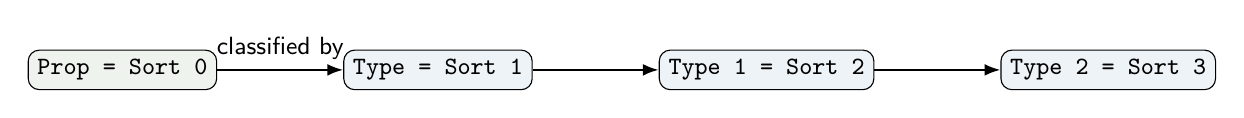
\begin{tikzpicture}[node distance=9mm and 16mm, every node/.style={font=\small\sffamily}]
\node[draw,rounded corners,fill=Panel] (p) {\term{Prop = Sort 0}};
\node[draw,rounded corners,fill=PanelBlue,right=of p] (t0) {\term{Type = Sort 1}};
\node[draw,rounded corners,fill=PanelBlue,right=of t0] (t1) {\term{Type 1 = Sort 2}};
\node[draw,rounded corners,fill=PanelBlue,right=of t1] (t2) {\term{Type 2 = Sort 3}};
\draw[-{Latex[length=2mm]},thick] (p) -- node[above]{classified by} (t0);
\draw[-{Latex[length=2mm]},thick] (t0) -- (t1);
\draw[-{Latex[length=2mm]},thick] (t1) -- (t2);
\end{tikzpicture}
\end{center}

\section{Lean's universes are non-cumulative}

Lean uses a countable hierarchy of \emph{non-cumulative} universes.  A type that inhabits \term{Type} is not automatically treated as an inhabitant of \term{Type 1}.  Universe-polymorphic definitions are instead instantiated at the required level.

This often surprises users familiar with cumulative systems.  The hierarchy still satisfies

\begin{leanblock}[Universes themselves inhabit the next universe]
#check Type
-- Type : Type 1

#check Type 1
-- Type 1 : Type 2
\end{leanblock}

but a small data type is not silently lifted into every larger universe.  Lean's universe parameters and \term{max}/\term{imax} expressions keep definitions reusable without cumulative coercions.

\section{Universe polymorphism}

A polymorphic identity should work for propositions, ordinary data, and higher-universe objects:

\begin{leanblock}[Sort-polymorphic identity]
def sid.{u} {α : Sort u} (x : α) : α := x
\end{leanblock}

The universe parameter \term{u} is instantiated at each use.  Constants store a list of universe parameters in their declaration and a list of universe arguments in each \term{Expr.const} occurrence.

Lean's internal universe levels are built from:

\begin{itemize}
\item \term{zero};
\item \term{succ u};
\item \term{max u v};
\item \term{imax u v};
\item named parameters;
\item elaboration metavariables.
\end{itemize}

Kernel expressions cannot retain level metavariables, just as they cannot retain term metavariables.

\section{The meaning of \texttt{imax}}

The universe of a dependent function type is

\[
\operatorname{imax}(u,v) =
\begin{cases}
0, & v=0,\\
\max(u,v), & v>0.
\end{cases}
\]

This special operation encodes the impredicativity of \term{Prop}.  If the codomain of a $\Pi$-type is a proposition, the whole dependent function type remains a proposition no matter how large the domain is:

\[
\Pi(A:\mathsf{Type}\;42),\,P(A) : \mathsf{Prop}.
\]

A proposition may quantify over objects from arbitrary universes without leaving \term{Prop}.  By contrast, a data-valued dependent function must live high enough to contain both its domain and codomain structure.

The pinned kernel implementation computes this literally: \term{infer_pi} collects domain sort levels and folds \term{mk_imax} from the final codomain level.

\section{Proof irrelevance}

All proofs of the same proposition are treated as definitionally equal by Lean's kernel.  If $p,q:P$ with $P:\mathsf{Prop}$, then the kernel's definitional equality can regard $p$ and $q$ as equal without comparing their proof structure.

Proof irrelevance supports efficient erasure and prevents programs from branching on which proof of a proposition was supplied.  It also explains why proposition-valued structures are not interchangeable with data-valued structures even when their constructor shapes match.

\section{Large elimination and restrictions}

Because \term{Prop} is impredicative and proof-irrelevant, arbitrary elimination from proposition-valued inductives into data would allow computational results to depend on erased proofs.  Lean therefore restricts such elimination, with special cases for subsingleton-like propositions.  One may eliminate \term{False} into any sort, but one may not generally turn an arbitrary existential proof into a data-level witness.

\begin{leantbox}
The Leant serializer records whether the goal itself is proposition-valued or data-valued and preserves distinctions among \term{And}/\term{Prod}/\term{PProd}, \term{Or}/\term{Sum}/\term{PSum}, and empty/unit families.  Djinn may search their common logical shape, but the renderer relies on Lean's expected type to recover the correct universe-specific constructor.
\end{leantbox}

\begin{sourcebox}
Universe syntax is defined in \url{https://github.com/leanprover/lean4/blob/79c4cd09fdab845aa6066bcbb09a663876601027/src/Lean/Level.lean}.  The kernel rules for sorts, applications, and $\Pi$ universes are implemented in \path{src/kernel/type_checker.cpp}.  The official reference explicitly describes Lean's universes as non-cumulative and \term{Type u} as \term{Sort (u+1)}.
\end{sourcebox}

\begin{recapbox}
Lean avoids \term{Type : Type} with a non-cumulative universe hierarchy.  \term{Prop} is \term{Sort 0}; data universes start at \term{Sort 1}.  The $\Pi$ universe uses \term{imax}, making \term{Prop} impredicative.  Proof irrelevance is a kernel conversion principle, not an optional theorem.
\end{recapbox}

\chapter{Computation and Definitional Equality}\label{ch:defeq}

\section{Two ways terms can be equal}

Lean distinguishes:

\begin{description}
\item[Definitional equality] $t \defeq u$: the type checker recognizes the terms as equal by built-in computation and conversion.  No proof object is required.
\item[Propositional equality] $h : t = u$: an explicit term inhabits the inductive equality proposition.
\end{description}

For example,

\[
(\lambda x.\,x+1)\;4 \defeq 5
\]

by beta reduction and natural-number computation.  Therefore \term{rfl} can prove an equality whose two sides reduce to the same normal form.

\begin{leanblock}[Computation makes reflexivity sufficient]
example : (fun x : Nat => x + 1) 4 = 5 := rfl
\end{leanblock}

\section{The main reduction rules}

\subsection{Beta reduction}

Applying a lambda substitutes the argument into the body:

\[
(\lambda x:A.\,t)\;a \longrightarrow t[a/x].
\]

\subsection{Delta reduction}

A transparent definition may unfold to its body:

\[
\mathsf{twice}\;f\;x \longrightarrow f(fx).
\]

The kernel uses lazy delta reduction and reducibility hints to decide an efficient unfolding order.  The hints affect performance, not the logical meaning of transparent definitions.

\subsection{Iota reduction}

A recursor or pattern match applied to a constructor reduces to the matching branch.  Informally:

\[
\mathsf{match}\;\mathsf{inl}\;a\;\mathsf{with}\;\cdots
\longrightarrow \text{left branch with }a.
\]

\subsection{Zeta reduction}

A \term{let} expression substitutes its value into the body:

\[
\mathsf{let}\;x:=a;\;t \longrightarrow t[a/x].
\]

\subsection{Projection reduction}

Projecting a field from a constructor reduces to that field.  Lean also supports eta-like conversion for functions and nonrecursive structures in the kernel's definitional equality procedure.

\section{Weak-head normalization}

The kernel rarely normalizes every subterm eagerly.  It computes to \emph{weak-head normal form}: enough to expose the outer constructor.  If a purported function type is hidden behind a definition, \term{ensure_pi} weak-head normalizes until it sees a $\Pi$ or reports an error.  If a purported sort is hidden, \term{ensure_sort} does the analogous work.

This strategy matters operationally.  Full normalization can be expensive; type checking usually needs only the head shape and selective definitional equality.

\section{Conversion in typing}

A conversion rule permits a term inferred at type $A$ to be used where a definitionally equal type $B$ is expected:

\begin{formalbox}[Conversion]
\[
\frac{
  \Gamma \vdash t : A
  \qquad
  A \defeq B
  \qquad
  \Gamma \vdash B : s
}{
  \Gamma \vdash t : B
}
\]
\end{formalbox}

Dependency makes this indispensable.  A recursive function may produce \term{Vector α (Nat.succ n)} while the expected type prints as \term{Vector α (n + 1)}; whether the terms align depends on reduction and the definitions involved.

\section{Opaque declarations and theorems}

Not every named constant unfolds.  Opaque definitions and theorem declarations expose their types but not reducible bodies to ordinary kernel conversion.  This modularity keeps checking stable and prevents proof terms from expanding uncontrollably.

A term can still use an opaque theorem as a constant.  What it cannot do is rely on computing through the theorem's hidden proof body.

\section{Why a renderer cannot implement definitional equality itself}

Leant's Haskell side sees strings, fragment trees, Djex types, and candidate graphs.  Reimplementing Lean's full conversion relation there would require reproducing environment lookup, universe instantiation, recursive recursors, projections, proof irrelevance, native reductions, and transparency behavior.  That would create a second, drifting authority.

Instead, Leant uses Lean's own metaprogramming operations during translation and Lean's own elaborator/kernel during verification.  Haskell-side normalization is limited to its own representations and never grants Lean type authority.

\begin{keyidea}[Expected-type elaboration is a semantic service]
A candidate such as \term{⟨x, y⟩} is intentionally incomplete as a standalone string.  Against an exact expected type, Lean selects a constructor, inserts universe parameters and implicit arguments, resolves notation, checks conversion, and produces a kernel expression.  Leant treats that elaboration as the authoritative final lowering pass.
\end{keyidea}

\begin{recapbox}
Definitional equality is computation built into type checking.  It includes beta, delta, iota, zeta, projections, proof irrelevance, and eta behavior implemented by the kernel's conversion algorithm.  Leant delegates this entire relation back to Lean instead of approximating it in Haskell.
\end{recapbox}

\chapter{Inductive Types, Recursors, and Termination}\label{ch:inductives}

\section{Data by constructors}

An inductive declaration introduces a type as the least collection closed under specified constructors:

\begin{leanblock}[Natural numbers]
inductive MyNat where
  | zero : MyNat
  | succ : MyNat → MyNat
\end{leanblock}

Every value of \term{MyNat} is built by a finite constructor tree.  This gives both a way to construct values and a complete way to consume them: handle \term{zero} and handle \term{succ n} assuming the recursive result for $n$.

\section{Parameters and indices}

A parameter is uniform across a whole inductive family.  An index may vary by constructor:

\begin{leanblock}[An indexed vector family]
inductive Vec (α : Type u) : Nat → Type u where
  | nil : Vec α 0
  | cons {n : Nat} : α → Vec α n → Vec α (n + 1)
\end{leanblock}

Here $\alpha$ is a parameter and the length is an index.  The constructors return different members of the family.  Pattern matching on a vector therefore refines what is known about its length.

The Lean kernel's \term{InductiveVal} explicitly records the number of parameters and indices, constructor names, universe parameters, whether the family is recursive, and other metadata used to construct and check recursors.

\section{Recursors are the primitive eliminators}

For each accepted inductive declaration, Lean generates a recursor.  For natural numbers, its shape is conceptually:

\[
\mathsf{Nat.rec} :
\Pi(motive : \mathsf{Nat}\to\mathsf{Sort}\;u),
\;motive\;0 \to
(\Pi n, motive\;n \to motive\;(n+1)) \to
\Pi n, motive\;n.
\]

The \emph{motive} is the result type family.  If it is constant, recursion returns ordinary data.  If it depends on the input, the same recursor performs induction or dependent pattern matching.

This one principle unifies:

\begin{itemize}
\item defining a numeric function by recursion;
\item proving a proposition by induction;
\item constructing an indexed result whose type tracks the input;
\item eliminating a sum or product by cases.
\end{itemize}

\section{Pattern matching is elaborated}

User-friendly equations and \term{match} expressions are compiled into recursors, auxiliary definitions, and equality transports.  The equation compiler is not trusted.  Its generated term is checked by the kernel against the declared type.

For a dependent match, each branch may have a refined expected type.  Consider a vector head operation that requires nonempty length:

\begin{leanblock}[Index refinement by pattern matching]
def Vec.head : Vec α (n + 1) → α
  | .cons a _ => a
\end{leanblock}

The impossible \term{nil} branch is absent because \term{Vec α 0} cannot unify with \term{Vec α (n + 1)}.

\section{Strict positivity}

Inductive definitions must satisfy positivity conditions.  Roughly, the type being defined may occur recursively only in positions that preserve monotonicity.  A forbidden negative occurrence would allow paradoxical self-application and destroy consistency.

Lean's inductive checker validates positivity, universe constraints, constructor result heads, and elimination restrictions before adding the compiled declarations to the environment.

\section{Termination and totality}

Lean's logical definitions must terminate.  Structural recursion is accepted when recursive calls are made on syntactically smaller constructor fields.  More general recursion can be compiled through well-founded recursion, requiring a proof that calls decrease according to a well-founded relation.

The kernel itself does not have a primitive ``general recursive definition'' constructor.  The source comments in \path{src/Lean/Declaration.lean} state that recursive definitions are compiled using recursors and \term{WellFounded.fix}.  Unsafe or partial definitions belong to separate safety classes and cannot be used to prove safe logical declarations as though they were total.

\section{Why recursive synthesis is a separate problem}

A type such as \term{List α → List α} does not say whether the result should recurse over the list, preserve length, reverse order, or ignore input.  Inventing a recursive program requires choosing:

\begin{itemize}
\item an eliminator or recursion scheme;
\item the argument on which to recurse;
\item branch bodies;
\item recursive-call arguments;
\item termination evidence;
\item possibly a dependent motive.
\end{itemize}

Leant therefore does not pretend that general recursive synthesis follows from propositional inhabitation.  It supports bounded constructor introduction for certain recursive types and can expose curated library functions as provider premises.  Recursive elimination is restricted and engine-specific; arbitrary recursor invention remains out of scope for ordinary \term{:synth}.

\begin{leantbox}[Constructor inventory is evidence]
For a nonrecursive, nonindexed inductive with explicit non-dependent fields, Leant may translate the declaration into a finite sum of products.  For a recursive type it records whether the constructor inventory is complete and how recursive occurrences appear.  An incomplete or ambiguous inventory may still help produce positive candidates, but it cannot justify a conclusive negative result.
\end{leantbox}

\begin{recapbox}
Inductive declarations generate constructors and recursors.  Parameters are uniform; indices vary and enable type refinement.  Pattern matching is compiled and checked.  Total recursion is reduced to structurally or well-foundedly justified terms.  General recursive synthesis is therefore much richer than propositional proof search.
\end{recapbox}

\chapter{Equality, Rewriting, and Transport}\label{ch:equality}

\section{Equality is an indexed inductive family}

Lean's propositional equality has one constructor:

\begin{leanblock}[Conceptual shape of equality]
Eq.refl : (a : α) → a = a
\end{leanblock}

The family \term{Eq a b} is indexed by both endpoints.  The constructor exists only when they are the same term, modulo definitional equality.

An equality proof can therefore refine types when eliminated.  This is much stronger than a Boolean comparison.

\section{Reflexivity and computation}

The tactic or term \term{rfl} constructs \term{Eq.refl _}.  It succeeds when both sides are definitionally equal:

\begin{leanblock}[Reflexivity after reduction]
example (x : Nat) : (fun y => y) x = x := rfl
example : List.length [10, 20] = 2 := rfl
\end{leanblock}

When equality is not definitional, one needs a theorem or a derivation using induction, congruence, rewriting, arithmetic, or another proof method.

\section{Transport}

If $h : a = b$ and $P : A \to \mathsf{Sort}\;u$, a value of $P(a)$ can be transported to $P(b)$:

\[
\mathsf{Eq.rec} : P(a) \to a=b \to P(b).
\]

Lean's rewrite notation hides this eliminator:

\begin{leanblock}[Transport across type equality]
def castValue {α β : Sort u} (h : α = β) (x : α) : β :=
  h ▸ x
\end{leanblock}

The term $x$ cannot be returned directly because its type is $\alpha$, not $\beta$.  The equality proof changes the expected type.

\section{Transport in indexed families}

Suppose $v : \mathsf{Vector}\;\alpha\;n$ and $h:n=m$.  Transport yields a vector at index $m$:

\begin{leanblock}[Changing an index with an equality]
def changeLength {n m : Nat} (h : n = m)
    (v : Vector α n) : Vector α m :=
  h ▸ v
\end{leanblock}

A synthesis engine that treats \term{Vector α n} and \term{Vector α m} as unrelated opaque atoms will not discover this term.  A synthesis engine that simply erases the indices and treats both as \term{Vector α} may generate unsound terms.  Correct dependent synthesis must reason about the equality and insert transport.

\section{Dependent pattern matching creates equalities implicitly}

When matching an indexed constructor, Lean refines the index and may insert transports behind the scenes.  The surface branch looks simple because the elaborator constructs the appropriate motive and equality reasoning.

This is a major line between Leant's \term{:synth} and \term{:prove} modes.  The former can transport an opaque dependent proposition as a whole if the surrounding logic only rearranges it.  It does not generally invent index equalities, dependent motives, or transport chains.  In proof mode, standard Lean tactics and user guidance can expose and solve those obligations.

\section{Homogeneous and heterogeneous equality}

Ordinary \term{Eq} compares terms of one common type.  Dependent developments sometimes need heterogeneous equality, where the endpoint types differ.  Lean provides tools such as \term{HEq}, but most practical reasoning reduces heterogeneous equalities to ordinary equality plus transport.

The presence of such relations is another warning against flattening dependent applications into nominal strings.  Their argument structure and universe instantiations determine what can be rewritten.

\begin{keyidea}[Dependency is not decoration]
An index in \term{Vector α n} can govern which constructors exist, which patterns are possible, and what result type a branch must produce.  Erasing the index changes the typing problem.  Keeping it only as an opaque identity preserves sound transport of whole values but sacrifices the ability to synthesize index-sensitive computations.
\end{keyidea}

\begin{recapbox}
Propositional equality is an indexed family whose eliminator performs transport.  \term{rfl} uses definitional equality; rewriting uses an explicit proof.  Indexed synthesis often requires equality generation and transport, which Leant intentionally does not model in its ordinary structural fragment.
\end{recapbox}

\chapter{The Calculus of Constructions and Its Inductive Extension}\label{ch:coc}

\section{Why the name matters}

The Calculus of Constructions (CoC) is a compact dependent lambda calculus in which terms, types, and type constructors inhabit one stratified language.  It combines:

\begin{itemize}
\item ordinary functions from terms to terms;
\item polymorphic functions from types to terms;
\item type operators from types to types;
\item dependent type families from terms to types.
\end{itemize}

Lean is based on a version of this tradition with a countable hierarchy of non-cumulative universes, an impredicative proof-irrelevant \term{Prop}, inductive types and recursors, quotient support, and a modern elaboration/programming infrastructure.  It is therefore better to say ``Lean's dependent type theory is in the CoC/CIC family'' than to identify it mechanically with one historical presentation.

\section{The lambda cube}

The lambda cube classifies typed lambda calculi by three independent forms of dependency added to the simply typed lambda calculus.  Let $*$ stand informally for ordinary types and \term{□} for kinds or universes.

\begin{center}
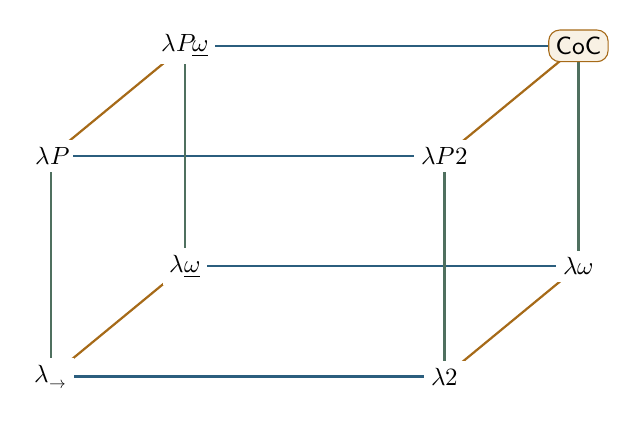
\begin{tikzpicture}[
  every node/.style={font=\small\sffamily,inner sep=2.5pt},
  vertex/.style={fill=white},
  poly/.style={draw=Blue,thick},
  dep/.style={draw=Sage,thick},
  typeop/.style={draw=Gold,thick}]
\coordinate (A) at (0,0);
\coordinate (B) at (5.0,0);
\coordinate (C) at (0,2.8);
\coordinate (D) at (5.0,2.8);
\coordinate (E) at (1.7,1.4);
\coordinate (F) at (6.7,1.4);
\coordinate (G) at (1.7,4.2);
\coordinate (H) at (6.7,4.2);

% Each edge color is one of the three independent lambda-cube axes.
\foreach \u/\v in {A/B,C/D,E/F,G/H} \draw[poly] (\u) -- (\v);
\foreach \u/\v in {A/C,B/D,E/G,F/H} \draw[dep] (\u) -- (\v);
\foreach \u/\v in {A/E,B/F,C/G,D/H} \draw[typeop] (\u) -- (\v);

\node[vertex] at (A) {$\lambda_{\to}$};
\node[vertex] at (B) {$\lambda 2$};
\node[vertex] at (C) {$\lambda P$};
\node[vertex] at (D) {$\lambda P2$};
\node[vertex] at (E) {$\lambda\underline{\omega}$};
\node[vertex] at (F) {$\lambda\omega$};
\node[vertex] at (G) {$\lambda P\underline{\omega}$};
\node[fill=PanelGold,draw=Gold,rounded corners] at (H) {CoC};
\end{tikzpicture}

\vspace{0.25em}
{\footnotesize\sffamily
\begin{tabular}{@{}ccc@{}}
\textcolor{Blue}{\rule{1.7em}{1.5pt}} &
\textcolor{Sage}{\rule{1.7em}{1.5pt}} &
\textcolor{Gold}{\rule{1.7em}{1.5pt}} \\
polymorphism & dependency & type operators \\
$\text{types}\to\text{terms}$ & $\text{terms}\to\text{types}$ & $\text{types}\to\text{types}$
\end{tabular}}
\end{center}

The top corner supports all three axes.  The ordinary $\Pi$-type constructor is expressive enough to encode them uniformly, with universes preventing paradox.

\section{What inductive types add}

Pure CoC has dependent functions but does not by itself provide the practical repertoire of freely generated datatypes and induction principles used in Lean.  The Calculus of Inductive Constructions (CIC) adds inductive families together with checked eliminators.

From the user's perspective, this supplies \term{Nat}, \term{List}, equality, conjunction, disjunction, existential quantification, structures, well-founded recursion infrastructure, and essentially every concrete datatype.

From the kernel's perspective, an inductive block is checked once and compiled into declarations for:

\begin{itemize}
\item the type former;
\item each constructor;
\item recursors and related eliminators;
\item no-confusion and projection machinery in higher layers as appropriate.
\end{itemize}

\section{A compact core grammar}

Ignoring literals, metadata, and projections, the dependent lambda-calculus core can be sketched as

\[
\begin{aligned}
t ::= {}& x
\mid \mathsf{Sort}\;u
\mid c.\{\bar u\}
\mid t\;t
\mid \lambda(x:A),t\\
&\mid \Pi(x:A),B
\mid \mathsf{let}\;x:A:=t;\,u.
\end{aligned}
\]

Lean's actual \term{Expr} datatype closely mirrors this grammar, plus free and meta variables, literals, metadata, and compact projections.  Inductive types do not require a new general expression constructor: they enter as constants and recursors stored in the environment.

\section{Normalization, consistency, and total programs}

The logical use of Curry--Howard depends on terms not conjuring inhabitants through nontermination.  In a language where an infinite loop can be assigned every type, every proposition would become ``provable'' by divergence.  Lean therefore separates safe total definitions from unsafe or partial computation.

Strong normalization is a central metatheoretic property of the pure calculi; Lean's implemented theory extends the core while preserving a small checkable proof language.  The practical guarantee is enforced syntactically and semantically through checked declarations, positivity, universe consistency, and termination compilation.

\section{Why Djinn does not search CoC directly}

Full proof search for arbitrary dependent type theory is qualitatively different from propositional inhabitation.  A searcher may need to invent:

\begin{itemize}
\item terms that appear inside types;
\item motives for dependent eliminators;
\item equality proofs and transports;
\item universe instantiations;
\item recursive definitions and termination proofs;
\item instances, coercions, overloaded notation, and environment-dependent constants.
\end{itemize}

There is no simple finite LJT-style decision procedure for all of that.  Leant's architecture is therefore a principled compromise: use Lean to understand and check the rich language; project an admitted structural fragment to search calculi with known operational properties; preserve unsupported dependent subterms as opaque, alpha-aware atoms; and fail closed on negative evidence.

\begin{leantbox}[The architecture follows the theory]
Leant is not missing a magical parser flag that would make Djinn ``support dependent types.''  The search calculus itself is propositional and its proof terms are untyped lambdas with tuple/sum operations.  Supporting dependency analytically would require a different proof calculus, candidate representation, unifier, eliminator search, and completeness argument.  Opaque cargo is a deliberate semantic boundary, not merely an unfinished pretty printer.
\end{leantbox}

\begin{recapbox}
CoC unifies ordinary functions, polymorphism, type operators, and dependent families.  CIC adds inductive families and recursors.  Lean belongs to this family but has its own precise universe, proof-irrelevance, quotient, safety, and implementation choices.  Djinn searches a much smaller propositional calculus, so Leant must mediate between two genuinely different logics.
\end{recapbox}


\part{How Lean Implements the Theory}\label{part:implementation}

\chapter{From Surface Syntax to a Kernel Term}\label{ch:elaboration}

\section{Lean source is intentionally incomplete}

Human-friendly Lean code omits information that the kernel requires.  Consider:

\begin{leanblock}[Compact surface syntax]
fun x => (x, x)
\end{leanblock}

The source does not state the type of $x$, the universe containing that type, the exact product constructor, or its implicit parameters.  In a suitable expected context, Lean can infer all of them.  Without an expected type, it may report an ambiguity.

This gap is filled by \emph{elaboration}: a constraint-generating and constraint-solving translation from syntax to fully explicit core expressions.

\section{The pipeline}

A simplified Lean command pipeline is:

\begin{center}
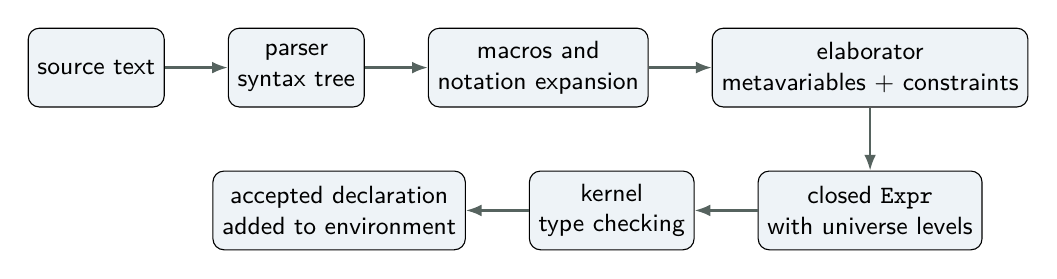
\begin{tikzpicture}[
  node distance=8mm and 8mm,
  box/.style={draw,rounded corners,minimum height=10mm,align=center,font=\small\sffamily,fill=PanelBlue},
  arr/.style={-{Latex[length=2mm]},thick,color=MutedInk}]
\node[box] (text) {source text};
\node[box,right=of text] (parser) {parser\\syntax tree};
\node[box,right=of parser] (macro) {macros and\\notation expansion};
\node[box,right=of macro] (elab) {elaborator\\metavariables + constraints};
\node[box,below=of elab] (expr) {closed \term{Expr}\\with universe levels};
\node[box,left=of expr] (kernel) {kernel\\type checking};
\node[box,left=of kernel] (env) {accepted declaration\\added to environment};
\draw[arr] (text) -- (parser);
\draw[arr] (parser) -- (macro);
\draw[arr] (macro) -- (elab);
\draw[arr] (elab) -- (expr);
\draw[arr] (expr) -- (kernel);
\draw[arr] (kernel) -- (env);
\end{tikzpicture}
\end{center}

Tactics, type-class resolution, coercion insertion, notation elaborators, and user metaprograms all operate before the final kernel check.  They may be complicated and occasionally buggy without becoming proof authorities: their output is rejected unless it forms a valid kernel term.

\section{Expected-type-directed elaboration}

Elaboration often proceeds bidirectionally:

\begin{itemize}
\item \emph{Synthesis mode}: infer a term's type from its syntax.
\item \emph{Checking mode}: elaborate a term against a known expected type.
\end{itemize}

A lambda with an omitted binder type is easy in checking mode:

\begin{leanblock}[Expected type supplies the binder]
example : Nat → Nat := fun x => x
\end{leanblock}

The expected $\mathsf{Nat}\to\mathsf{Nat}$ tells the elaborator that $x:\mathsf{Nat}$ and that the body must produce a natural number.

Anonymous constructor syntax is similarly expected-type dependent:

\begin{leanblock}[One syntax, several possible constructors]
example (p : P) (q : Q) : P ∧ Q := ⟨p, q⟩
example (a : A) (b : B) : A × B := ⟨a, b⟩
\end{leanblock}

The string \term{⟨p, q⟩} does not name \term{And.intro} or \term{Prod.mk}.  The expected type decides.

\section{Unification and metavariable assignment}

Suppose \term{id} has type \term{{α : Sort u} → α → α}.  When elaborating \term{id 5}, Lean creates unknowns for the universe and $\alpha$, then unifies the explicit argument's type \term{Nat} with $\alpha$.  The solved term is conceptually \term{id.{1} (α := Nat) 5}, though the printed term remains concise.

Dependent unification is more subtle because metavariables may occur inside types.  Lean combines higher-order pattern unification, reduction, postponement, and specialized elaboration procedures rather than solving arbitrary higher-order unification, which is undecidable.

\section{Implicit arguments and placeholders}

Implicit parameters are inserted automatically when a constant is applied.  A placeholder \term{_} asks Lean to create a metavariable explicitly.  This is useful to Leant's renderer:

\begin{leanblock}[A reconstruction placeholder]
provider _ x
\end{leanblock}

The search engine may know that a provider should be applied but may not have retained a surface-level explicit type argument.  Emitting \term{_} delegates that choice to the exact Lean environment.  If inference is ambiguous or inconsistent, candidate verification fails.

\section{Type classes are ordinary dependent parameters plus search}

A class declaration defines a structure.  An instance is a term of that structure type.  A binder \term{[C α]} is an instance-implicit dependent function argument.  The elaborator invokes type-class resolution to synthesize it.

\begin{leanblock}[Dictionary passing beneath surface syntax]
class Render (α : Type u) where
  render : α → String

def showOne {α : Type u} [Render α] (x : α) : String :=
  Render.render x
\end{leanblock}

Conceptually, \term{showOne} receives a dictionary carrying the \term{render} operation.  That dictionary is a real value and may contain computational content.  Erasing it from a synthesis problem is therefore harmless only under carefully restricted conditions.

\begin{leantbox}[Hidden dictionaries poison negative evidence]
A generated candidate can often leave instance arguments implicit and let Lean resolve them.  But a claim that no inhabitant exists cannot ignore a hidden instance premise: the dictionary may provide exactly the operation or value needed to construct the result.  Leant records instance binders and refuses strong refutation when their evidence was not represented exhaustively.
\end{leantbox}

\section{Coercions and overloaded notation}

Numerals, arithmetic operators, field notation, sequence literals, and many other surface forms are overloaded.  Their elaboration depends on expected types and instances.  A numeral \term{0} may elaborate as a natural number, integer, rational, finite-ring element, or user-defined type through \term{OfNat}.

This is another reason candidate verification must compile the exact source text in context.  A Haskell renderer cannot decide the meaning of every Lean notation independently of imports and instances.

\section{Auto-implicit names}

With \term{autoImplicit true}, an undeclared identifier in a declaration header may be introduced as an implicit variable when Lean can infer an appropriate kind.  Leant's verification command deliberately enables the option because synthesized goals and user sessions may rely on the same convention.

The option affects elaboration, not kernel semantics.  The resulting declaration still contains explicit binders and universe parameters in its core type.

\begin{warningbox}[Elaboration success is stronger than parsing, weaker than behavioral correctness]
A candidate that parses may still fail to resolve names, infer parameters, solve instances, or satisfy the expected type.  A candidate that elaborates and kernel-checks is a genuine inhabitant of the goal.  It may nevertheless be the wrong inhabitant for the user's unstated behavioral intent.
\end{warningbox}

\begin{recapbox}
Lean source relies on expected types, metavariables, unification, implicit arguments, type-class search, coercions, and notation elaborators.  The output is a fully explicit kernel expression.  Leant intentionally emits syntax that Lean must elaborate, because that is the only reliable way to recover exact environment-dependent details.
\end{recapbox}

\chapter{The Kernel Representation: \texttt{Level}, \texttt{Expr}, and \texttt{Declaration}}\label{ch:kernel-expr}

\section{Universe levels}

The datatype \term{Lean.Level} represents universe expressions:

\begin{center}
\begin{tabularx}{\textwidth}{@{}l X X@{}}
\toprule
Constructor & Meaning & Typical source form \\
\midrule
\term{zero} & level $0$ & \term{Prop} \\
\term{succ u} & successor & \term{Type u} uses \term{succ u} \\
\term{max u v} & maximum & universe of data-valued combinations \\
\term{imax u v} & impredicative maximum & universe of a dependent product \\
\term{param n} & declaration universe parameter & \term{.{u}} \\
\term{mvar id} & unsolved elaboration level & temporary only \\
\bottomrule
\end{tabularx}
\end{center}

Level expressions are normalized and compared modulo their algebraic meaning.  A closed kernel declaration may mention named parameters but not unresolved level metavariables.

\section{The expression datatype}

At the pinned Lean revision, the core expression datatype has the following constructors:

\begin{longtable}{@{}>{\ttfamily}l >{\raggedright\arraybackslash}p{0.24\textwidth} >{\raggedright\arraybackslash}p{0.52\textwidth}@{}}
\toprule
\normalfont Constructor & \normalfont Role & \normalfont Important detail \\
\midrule
\endfirsthead
\toprule
\normalfont Constructor & \normalfont Role & \normalfont Important detail \\
\midrule
\endhead
bvar & bound variable & de Bruijn index into surrounding binders \\
fvar & free variable & stable identifier backed by a local-context declaration \\
mvar & metavariable & elaboration hole; rejected by the kernel \\
sort & universe term & \term{Prop}, \term{Type u}, and general \term{Sort u} \\
const & global constant & exact name plus universe arguments \\
app & application & applications are left-nested binary nodes \\
lam & lambda abstraction & name hint, domain, body, binder information \\
forallE & dependent product & represents both $\Pi$ and non-dependent arrow \\
letE & local definition & declared type, value, body, and nondependency flag \\
lit & literal & natural or string literal with kernel reduction support \\
mdata & metadata wrapper & definitionally equal to the wrapped expression \\
proj & structure projection & type name, field index, and structure expression \\
\bottomrule
\end{longtable}

This is strikingly small.  There is no kernel node for \term{if}, \term{match}, \term{structure}, theorem tactics, notation, list syntax, or type classes.  Those are elaborated into applications of constants, lambdas, $\Pi$-types, recursors, and projections.

\section{One constructor for arrows and quantifiers}

The expression

\begin{leanblock}[A non-dependent arrow]
Nat → Bool
\end{leanblock}

and the expression

\begin{leanblock}[A dependent universal]
(n : Nat) → Fin (n + 1)
\end{leanblock}

both elaborate to \term{forallE}.  The body of the first does not contain the bound variable; the body of the second does.  Surface \term{∀} is also the same node.

This single fact explains much of Leant's serializer complexity: it must inspect domain sorts, binder visibility, body dependency, application heads, and local variable roles to classify a Lean $\Pi$ into Djex-compatible type quantification, value implication, opaque dependency, or instance evidence.

\section{Applications are spines}

The term \term{f a b c} is represented as

\[
(((f\;a)\;b)\;c).
\]

Utilities recover the head and argument array.  Leant uses this view to recognize named logical families such as \term{And P Q}, nominal type-constructor applications, class heads, and inductive family applications.

A dependent application cannot be classified solely by its printed head.  Its arguments may be types, values, indices, proofs, or universe-polymorphic terms.  The serializer asks Lean for each argument's type and whether the whole application is itself type-valued.

\section{Bound and free variables}

Inside stored declarations, lambda and $\Pi$ bodies use de Bruijn bound variables.  Metaprograms often open a binder by creating a fresh free variable, adding its declaration to the local context, and instantiating the body.  This makes its type and binder metadata available through ordinary APIs.

Leant's generated serializer follows that pattern when traversing dependent foralls and provider schemes.  The emitted fragment uses explicit string identities, but those strings are allocated under alpha-aware discipline rather than copied naïvely from pretty-printed binder names.

\section{Declarations and environments}

The global environment maps names to checked declaration records.  Major declaration categories include:

\begin{itemize}
\item axioms;
\item transparent definitions;
\item theorems;
\item opaque definitions;
\item quotient primitives;
\item inductive declarations and their compiled constants;
\item unsafe, partial, and mutual definitions used under restricted safety rules.
\end{itemize}

A constant occurrence stores only its name and universe arguments.  The environment supplies its type, value if reducible, safety information, and inductive metadata.

This environment dependence is why a bare goal string is not a complete synthesis problem.  The same spelling can resolve differently under namespaces and imports; constructors and providers available in one session may not exist in another; instances alter elaboration; reducible definitions change visible structure.

\section{Inductive metadata}

For an inductive family, the environment records parameters, indices, constructors, recursion status, universe parameters, and recursor information.  Leant queries this live metadata instead of trying to infer constructors from names or printed declarations.

The distinction among parameter, index, and dependent constructor field is semantic:

\begin{itemize}
\item parameters may be carried uniformly into an expanded nominal family;
\item indices generally force the family to remain opaque;
\item non-dependent explicit fields may become product components;
\item recursive occurrences require bounded and inventory-aware handling;
\item hidden or dependent fields prevent an exact first-order sum-of-products translation.
\end{itemize}

\begin{sourcebox}
The exact expression constructors and locally nameless design are documented in \url{https://github.com/leanprover/lean4/blob/79c4cd09fdab845aa6066bcbb09a663876601027/src/Lean/Expr.lean}.  Universe levels are in \path{src/Lean/Level.lean}; declaration records and inductive metadata are in \path{src/Lean/Declaration.lean}.  Kernel inference and definitional equality are in \path{src/kernel/type_checker.cpp}.
\end{sourcebox}

\begin{recapbox}
Lean's trusted term language is small: levels, variables, sorts, constants, applications, lambdas, dependent products, lets, literals, metadata, and projections.  Rich surface constructs become these nodes plus environment declarations.  Leant translates from this exact semantic representation, not from pretty-printed Lean text.
\end{recapbox}

\chapter{Trust, Tactics, Metaprograms, and Execution}\label{ch:trust}

\section{The small-kernel architecture}

Lean's trust story separates \emph{finding} a proof from \emph{checking} it.  The kernel is responsible for:

\begin{itemize}
\item checking universe levels and declaration parameters;
\item inferring expression types;
\item verifying applications and dependent substitution;
\item checking definitional equality;
\item validating inductive declarations and recursors;
\item enforcing safety boundaries on declarations.
\end{itemize}

The parser, macro system, elaborator, tactic framework, simplifier, compiler, and external automation may all be larger.  They are proof-producing or term-producing infrastructure.  A bug can cause failure, poor diagnostics, or a rejected term; it should not make an invalid term kernel-valid.

\section{Tactics are metaprograms over goals}

A tactic state contains metavariable goals.  A tactic may:

\begin{itemize}
\item introduce a binder;
\item apply a theorem and create subgoals;
\item refine a goal with a partially specified expression;
\item normalize or rewrite its target;
\item invoke search or decision procedures;
\item assign solved metavariables.
\end{itemize}

When no goals remain, the assigned expression is submitted through the ordinary checking path.  Tactics do not add a second notion of proof.

Leant's \term{:prove} command can be understood at this level: it interacts with a live proof state, asks its synthesis machinery for suitable terms at selected goals, and returns suggestions that Lean checks in context.

\section{Metaprogramming inside Lean}

Lean exposes APIs for expressions, local contexts, environments, declaration lookup, weak-head normalization, unification, instance synthesis, and syntax construction.  Leant uses generated Lean metaprograms to perform tasks that must respect the exact Lean semantics:

\begin{itemize}
\item elaborate the raw goal;
\item inspect the resulting \term{Expr};
\item classify logical connectives and $\Pi$ binders;
\item inspect inductive declarations and constructor fields;
\item discover provider constants from the live environment;
\item serialize a bounded semantic fragment to an S-expression.
\end{itemize}

The Haskell process does not link against Lean's internal objects directly.  It sends commands to a persistent Lean REPL worker and receives structured JSON responses containing messages, environment identifiers, and results.

\section{Axioms and opaque constants}

An axiom is a trusted assumption because no body is checked.  Quotient primitives and choice-related constants are part of Lean's foundational environment design.  Imported projects may add their own axioms.

An opaque theorem is different: its body was checked when declared, but later conversion does not unfold it.  Both appear as constants during downstream checking, yet their provenance differs.  \texttt{\#print axioms} follows dependencies to report axiomatic assumptions.

\section{Proof irrelevance and erasure}

Terms whose types lie in \term{Prop} are computationally irrelevant.  The compiler may erase them.  This permits specifications to carry proofs without runtime cost, but it constrains elimination from \term{Prop} into data.

The kernel still type checks proof arguments before erasure.  A generated program cannot bypass a required proof merely because it will not exist at runtime.

\section{Safe, unsafe, and partial definitions}

Lean is also a practical programming language.  It allows unsafe and partial definitions for executable code, but logical declarations are prevented from depending on unsafe computation as if it were a total proof-producing function.  The kernel source checks definition safety when constants are used.

Leant's candidate-verification command is marked \term{noncomputable} so candidates may use logically valid noncomputable constants without requesting executable code generation.  This relaxes compilation requirements, not type checking, universe checking, or safety checking.

\section{External solvers and replay}

An external solver can be used in several trust arrangements:

\begin{enumerate}
\item trust the solver's yes/no answer directly;
\item demand a certificate and check it in Lean;
\item reconstruct a proof term and ask the kernel to check it;
\item use the solver only as a heuristic or counterexample finder, then independently replay the result.
\end{enumerate}

Leant's ordinary Djex candidates use arrangement 3 at the final boundary: a Lean term is reconstructed and checked.  The optional Length/Z3 layer uses arrangement 4 for its bounded behavioral claims: the solver status alone is not authority; models and positive results are interpreted under a sealed contract and independently replayed by Djex's semantic layer.  Even then, the result is not automatically a general Lean theorem about extensional behavior.

\begin{keyidea}[Three different authorities]
\begin{enumerate}
\item Lean's kernel authorizes ``this term has this Lean type.''
\item A complete Djinn search over an exact fragment can authorize ``this translated formula has no proof.''
\item A sealed behavioral checker can authorize only the specific bounded semantic verdict described by its contract and replay rules.
\end{enumerate}
No one authority silently upgrades another.
\end{keyidea}

\begin{recapbox}
Lean's automation constructs terms; the kernel checks them.  Metaprograms can inspect the exact live environment without joining the trusted base.  Noncomputability, opacity, axioms, unsafe code, and external solvers each have distinct trust meanings.  Leant's design is strongest where it preserves those distinctions explicitly.
\end{recapbox}


\part{Leant and Djex}\label{part:leant}

\chapter{Djex's Deliberately Smaller Type World}\label{ch:djex-world}

\section{Why an intermediate language exists}

Lean's kernel language is compact, but its types are still fully dependent and environment-sensitive.  Searching that language directly would require solving the general problems described in Chapter~\ref{ch:coc}.  Djex instead provides synthesis engines for a Haskell-like source type language and, beneath Djinn, a propositional proof calculus.

Leant therefore needs an intermediate semantic boundary.  It cannot pass an arbitrary Lean \term{Expr} to Djex and hope that both sides mean the same thing.  It first classifies the goal into a Leant-owned fragment, then the engine adapter lowers admitted pieces into Djex representations.

\section{Djex's shared source type}

The current shared datatype \term{Language.Haskell.Synthesis.Type.Type} has these principal forms:

\begin{center}
\begin{tabularx}{\textwidth}{@{}l X X@{}}
\toprule
Djex constructor & Meaning & Lean relationship \\
\midrule
\term{TypeVariable} & type variable & a selected sort-bound Lean variable \\
\term{TypeConstructor} & nominal type constructor & a Lean constant retained by exact name mapping \\
\term{TypeApplication} & left-associated type application & only admitted type-level applications \\
\term{FunctionType} & non-dependent value arrow & a Lean $\Pi$ whose body does not depend on the value binder \\
\term{TupleType} & structural boxed/unboxed tuple & product-like fragment \\
\term{ForallType} & type-variable binders, class context, body & selected Lean sort quantifiers and exact provider schemes \\
\bottomrule
\end{tabularx}
\end{center}

This language supports polymorphism, higher-kinded constructor applications, constraints, tuples, and ordinary functions.  It has no constructor whose codomain is an arbitrary term-dependent type.  A \term{FunctionType A B} cannot express $\Pi(x:A),B(x)$ when $x$ appears in $B$.

The shared kind language is correspondingly Haskell-like:

\[
\mathsf{ProperTypeKind}
\quad\mid\quad
\mathsf{KindVariable}\;k
\quad\mid\quad
\mathsf{FunctionKind}\;k_1\;k_2.
\]

A sealed checked environment uses ground kinds with no unresolved kind variables.  Universe levels are not represented as Lean universes; the frontend must establish that the admitted source type has a compatible kind shape.

\section{Flexible variables and rigid variables}

Djex distinguishes inference variables that unification may instantiate from rigid skolems that must remain fixed:

\begin{itemize}
\item a \emph{flexible variable} represents an unknown chosen by the search/unifier;
\item a \emph{rigid variable} represents a universally quantified type that search must treat parametrically.
\end{itemize}

Confusing the two would make polymorphic synthesis unsound.  A target such as $\forall A\,B, A\to B$ must not be solved by unifying the rigid $A$ and $B$.

Djex's shared layer also owns capture-avoiding substitution, binder freshening, alpha normalization, validation, constructor-application normalization, and explicit forall-spine processing.  These are not cosmetic utilities: they enforce the source calculus on which both engines agree.

\section{Djinn's propositional formula language}

Djinn lowers types further into LJT formulas:

\[
F ::= P
\mid F \to F
\mid \bigwedge_i F_i
\mid \bigvee_i F_i
\mid \bot_N.
\]

The exact Haskell constructors are \term{PVar}, implication, n-ary \term{Conj}, constructor-tagged \term{Disj}, and nominal \term{Empty}.  A formula atom can be an ordinary symbol or an \term{OpaqueTypeSymbol} carrying an exact shared source type plus an alpha-normal key.

The proof-term language contains:

\begin{itemize}
\item variables, lambdas, and applications;
\item tuple construction and splitting;
\item sum injection and case analysis;
\item constructor descriptors carrying names and arities.
\end{itemize}

It is deliberately not a dependent proof-term language.  Formula atoms have no eliminators except those supplied by assumptions whose formulas expose implications, products, or sums.

\section{Opaque atoms preserve identity, not internal logic}

Suppose Leant encounters the Lean proposition \term{∀ n : Nat, P n}.  If the surrounding goal only needs to move this proposition from one product component to another, Djinn need not understand the quantifier.  It can represent the whole type as one atom $X$ and prove

\[
X \land Q \to Q \land X.
\]

The atom must still have stable semantic identity.  Comparing pretty-printed strings is unsafe because alpha-equivalent binders may print differently, distinct names may print similarly under namespaces, and renderer choices are not logical keys.  Djex's opaque symbol stores a structural source type and compares its alpha-normal key.

\begin{keyidea}[Opaque means indivisible, not forgotten]
An opaque atom retains enough identity to recognize the same type again and to reconstruct the original Lean spelling.  Search may copy it, pass it to a premise, return it, or place it in a product.  Search may not inspect its quantifiers, indices, equalities, or constructors.
\end{keyidea}

\section{The revision boundary}

The Leant snapshot studied here vendors Djex commit \DjexPinnedCommit\ as a submodule.  The standalone Djex repository was also inspected at \DjexCommit\ to understand the current shared architecture and documentation.  Statements about Leant's actual executable behavior should be read against the vendored revision; later standalone changes do not automatically enter Leant until the submodule pointer advances.

\begin{sourcebox}
The shared type and kind representations are in \url{https://github.com/VladimirReshetnikov/Djex/blob/0cf82f2aa22debb1de2c7aaa13a2abbe190550d8/synthesis/src/Language/Haskell/Synthesis/Type.hs} and \path{synthesis/src/Language/Haskell/Synthesis/Kind.hs}.  Djinn formulas and proof terms are in \path{djinn/src-core/Djinn/Internal/LJTFormula.hs}.
\end{sourcebox}

\begin{recapbox}
Djex does not contain Lean's dependent type theory.  Its shared source language is polymorphic and Haskell-like; Djinn's core is propositional.  Opaque atoms preserve exact alpha-aware identity while withholding internal structure.  Leant must prove, query by query, which Lean structure can safely cross this boundary.
\end{recapbox}

\chapter{The End-to-End Leant Pipeline}\label{ch:pipeline}

\section{A GHCi-shaped frontend for a Lean worker}

Leant is a Haskell executable that presents a persistent interactive session.  It feels like a REPL, but the authoritative Lean state lives in a separate Lean process.  Leant launches the community Lean REPL through a Lake environment and communicates over a blank-line-delimited JSON protocol.

The Haskell state tracks, among other things:

\begin{itemize}
\item current Lean environment identifiers;
\item replayable command history and session snapshots;
\item synthesized \term{it}, \term{it1}, \term{it2}, \dots{} bindings;
\item engine selection, step/queue/budget settings, and result quota;
\item provider inventories and cache keys tied to the Lean environment;
\item library, classical, and optional behavioral settings;
\item proof-mode state.
\end{itemize}

The persistent worker matters because a synthesis query is evaluated in the live environment created by previous commands and imports, not in a freshly guessed module.

\section{The major stages}

A representative \term{:synth GOAL} request follows this path:

\begin{center}
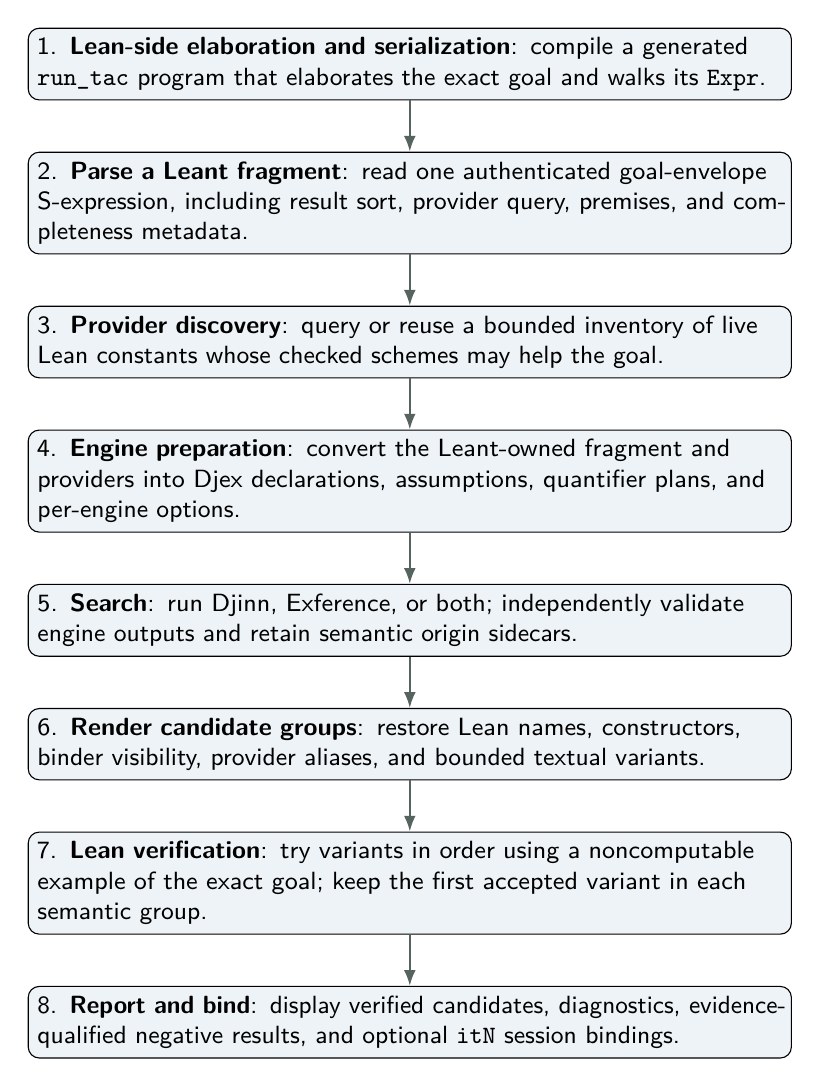
\begin{tikzpicture}[
  node distance=6.5mm,
  stage/.style={draw,rounded corners,align=left,font=\small\sffamily,
    text width=0.78\textwidth,minimum height=8mm,fill=PanelBlue},
  arr/.style={-{Latex[length=2mm]},thick,color=MutedInk}]
\node[stage] (s1) {1. \textbf{Lean-side elaboration and serialization}: compile a generated \term{run_tac} program that elaborates the exact goal and walks its \term{Expr}.};
\node[stage,below=of s1] (s2) {2. \textbf{Parse a Leant fragment}: read one authenticated goal-envelope S-expression, including result sort, provider query, premises, and completeness metadata.};
\node[stage,below=of s2] (s3) {3. \textbf{Provider discovery}: query or reuse a bounded inventory of live Lean constants whose checked schemes may help the goal.};
\node[stage,below=of s3] (s4) {4. \textbf{Engine preparation}: convert the Leant-owned fragment and providers into Djex declarations, assumptions, quantifier plans, and per-engine options.};
\node[stage,below=of s4] (s5) {5. \textbf{Search}: run Djinn, Exference, or both; independently validate engine outputs and retain semantic origin sidecars.};
\node[stage,below=of s5] (s6) {6. \textbf{Render candidate groups}: restore Lean names, constructors, binder visibility, provider aliases, and bounded textual variants.};
\node[stage,below=of s6] (s7) {7. \textbf{Lean verification}: try variants in order using a noncomputable example of the exact goal; keep the first accepted variant in each semantic group.};
\node[stage,below=of s7] (s8) {8. \textbf{Report and bind}: display verified candidates, diagnostics, evidence-qualified negative results, and optional \term{itN} session bindings.};
\foreach \a/\b in {s1/s2,s2/s3,s3/s4,s4/s5,s5/s6,s6/s7,s7/s8}
  \draw[arr] (\a) -- (\b);
\end{tikzpicture}
\end{center}

\section{Why translation happens inside Lean}

The serializer is emitted as Lean source and executed in the live worker.  It can therefore:

\begin{itemize}
\item elaborate the user's exact text with Lean's parser, macros, notation, imports, and options;
\item instantiate metavariables and weak-head normalize under Lean's definitions;
\item inspect \term{Expr.forallE} dependency and binder information;
\item resolve constant names and universe instantiations;
\item inspect inductive declarations and constructor types;
\item distinguish classes, propositions, data sorts, local variables, and nominal applications;
\item use Lean's definitional equality when comparing provider assignments.
\end{itemize}

Attempting these tasks by parsing pretty-printed goals in Haskell would immediately lose binding identity, namespace resolution, implicit arguments, reducible definitions, and universe information.

\section{The serializer output is treated as an untrusted protocol}

The generated Lean program emits a tagged S-expression inside an info message.  User code can also emit messages, so Leant does not trust the first line with a familiar prefix.  The parser requires exactly one well-formed goal envelope and rejects missing, duplicate, malformed, or trailing data.

This is a small but representative security principle: a semantic stage hands structured data to the next stage through a narrow checked boundary.  Messages, strings, and debug output never become authority merely because they resemble internal protocol text.

\section{Semantic origin survives textual operations}

A candidate is not only a string.  Leant records the exact source goal, search goal, declarations, providers, constructor/name maps, premise layout, engine preparation, search policy, and typed candidate or proof provenance needed to interpret it.

Rendering can produce several strings from one candidate.  Textual deduplication can merge equal display forms.  Verification can accept only one variant.  Through those operations, the semantic origin sidecar must remain attached to the group that owns it.  The internal documentation calls this a semantic-origin record; typed candidates additionally carry graph fingerprints and sealed inventories.

\begin{warningbox}[Authority does not transfer by string equality]
Two identical Lean strings generated from different environments or candidate graphs are not automatically the same semantic artifact.  A copied string has no right to inherit a completeness proof, behavioral contract, provider inventory, or solver receipt from another candidate merely because the characters match.
\end{warningbox}

\section{Backend verification usually dominates latency}

Structural search can be fast, especially for small formulas.  Candidate verification invokes Lean elaboration in the live environment for each variant and can dominate wall-clock time.  Leant therefore groups variants, uses lazy quota-aware verification, caches stable provider inventories, and avoids counting failed variants against the accepted-result quota.

\begin{sourcebox}
The process protocol and lifetime management are in \url{https://github.com/VladimirReshetnikov/Leant/blob/49c8f9f100a644b5a32b3c942bc6565a3a3ba6a0/src/Leant/Backend.hs}.  The interactive orchestration is in \path{src/Main.hs}.  Translation and verification command generation are in \path{src/Leant/Synth/Fragment.hs}; internal provenance invariants are summarized in \path{docs/synth-internals.md}.
\end{sourcebox}

\begin{recapbox}
Leant is a persistent Haskell controller around an authoritative Lean worker.  The goal is elaborated and classified inside Lean, searched in Djex, reconstructed in Haskell, and checked again inside Lean.  Structured origins and exact environment identities survive every intermediate transformation.
\end{recapbox}

\chapter{The Leant Synthesis Fragment}\label{ch:fragment}

\section{A frontend-owned semantic tree}

Leant does not translate Lean expressions directly into Djex types.  It first constructs its own \term{Frag} tree.  This keeps Lean-specific policy out of Djex and makes the exact/opaque/completeness decisions inspectable before an engine is chosen.

The principal fragment forms at the pinned revision are summarized below.

\begin{longtable}{@{}>{\ttfamily}l >{\raggedright\arraybackslash}p{0.26\textwidth} >{\raggedright\arraybackslash}p{0.50\textwidth}@{}}
\toprule
\normalfont Fragment & \normalfont Meaning & \normalfont Typical Lean source \\
\midrule
\endfirsthead
\toprule
\normalfont Fragment & \normalfont Meaning & \normalfont Typical Lean source \\
\midrule
\endhead
FArr & implication/function arrow & non-dependent \term{A → B} \\
FProd & logical product & \term{And}, structural proof product \\
FLeanProd & Lean data product & \term{Prod}/\term{PProd} distinction retained for rendering \\
FSum & logical/data sum & \term{Or}, \term{Sum}, or \term{PSum} with constructor map \\
FTop & unit/truth & \term{True}, \term{Unit}, \term{PUnit} \\
FBot & empty/falsity & \term{False}, \term{Empty}, \term{PEmpty} \\
FAll & admitted sort quantifier & type/sort binder plus explicitness flag \\
FInst & instance binder wrapper & hidden class evidence retained as a semantic boundary \\
FExactContext & structured class context & exact provider schemes/assignments only \\
FVar & universal type variable & selected sort-bound local variable \\
FAtom & opaque atom with refutation-safety bit & dependent or unsupported closed subtree \\
FApp & nominal/variable type application & first-order type-valued application with retained arguments \\
FParamInd & parameterized nonrecursive inductive & complete sum-of-products family with parameters \\
FInd & nonparameterized nonrecursive inductive & complete constructor inventory \\
FParamRec & parameterized recursive family & bounded recursive description plus inventory completeness \\
FRec & recursive family & bounded recursive description plus inventory completeness \\
FDepth & bounded-depth sentinel & marks a traversal limit rather than logical structure \\
\bottomrule
\end{longtable}

The exact constructor names matter less than the separation of concerns: arrows/products/sums are searchable logic; variables and applications preserve type structure; inductive records preserve declarations; atoms preserve identity; flags preserve whether absence of a proof can be trusted.

\section{Recognized logical structure}

The Lean-side traversal recognizes common families by exact constant identity, not by pretty-printed notation.  It structurally exposes:

\begin{itemize}
\item non-dependent arrows;
\item \term{And}, \term{Prod}, and \term{PProd};
\item \term{Or}, \term{Sum}, and \term{PSum};
\item \term{Iff}, lowered to the two implications;
\item \term{Not}, lowered to implication into falsity;
\item \term{False}/\term{Empty}/\term{PEmpty};
\item \term{True}/\term{Unit}/\term{PUnit};
\item selected sort quantifiers;
\item qualifying inductive declarations.
\end{itemize}

The renderer later restores nominal distinctions and exact constructor names.  The search engines can reason over a common product/sum structure without pretending the Lean families are definitionally identical.

\section{Non-dependent versus dependent foralls}

For a Lean \term{forallE}, the serializer asks whether the body contains the bound variable.

\begin{description}
\item[Non-dependent value binder] Becomes an arrow: introduce an ordinary term and synthesize the codomain.
\item[Sort-bound dependent binder] May become \term{FAll}: treat the bound object as a rigid type/sort variable and translate the body under it.
\item[Instance-implicit binder] Becomes \term{FInst} or exact context metadata under narrowly admitted provider rules.
\item[Other dependent value binder] Cannot become an ordinary arrow.  The whole type or affected subtree is sealed as an opaque atom.
\end{description}

Thus \term{∀ α : Type, α → α} can be represented as polymorphism, while \term{∀ n : Nat, P n} is not analyzed as a first-order type scheme.  It may still be carried opaquely.

\section{Type applications retain arguments when they are type-level}

Earlier versions of many synthesis adapters flatten applications into strings.  Leant instead retains the application head and argument fragments when Lean establishes that the application is type-valued and its arguments fit the admitted first-order kind discipline.

For example, \term{List α}, \term{Except ε α}, or a user-defined unary type constructor can preserve nominal family identity and parameter structure.  This supports higher-kinded provider matching and prevents unrelated instantiations from collapsing into one atom.

A term-indexed application such as \term{Vector α n} is different: $n$ is data, not a type parameter.  Unless the whole family is handled through a qualifying inductive representation, the application remains opaque.  The search engine does not erase $n$ and pretend all vector lengths coincide.

\section{Opaque dependent cargo}

Consider:

\begin{leanblock}[A dependent proposition moved as a whole]
opaque P : Nat → Prop
opaque Q : Prop

-- Synthesis target:
((∀ n : Nat, P n) ∧ Q) → Q ∧ (∀ n : Nat, P n)
\end{leanblock}

Let $X$ denote the exact opaque atom for \term{∀ n, P n}.  The searchable formula is

\[
(X \land Q) \to (Q \land X).
\]

Djinn can synthesize the product swap.  The renderer restores the original dependent formula as the type of the moved hypothesis; no term inspects $n$ or proves any \term{P n}.

This technique is useful for arbitrarily complicated formulas when their role is purely structural.  It is not dependent proof search.  A target such as

\begin{leanblock}[Requires analysis, not transport]
(∀ n : Nat, P n) → P 0
\end{leanblock}

requires instantiating the dependent function at $0$.  Whether Leant can handle a bounded form depends on its quantified-instantiation support and exact fragment plan; merely sealing the premise as one atom would make the needed application invisible.

\section{Refutation-safety bits}

An opaque atom can be safe for positive transport yet unsafe for negative reasoning.  Leant attaches a Boolean safety classification to atoms and applications.

A formula built only from universally quantified abstract variables can sometimes be treated parametrically: its hidden structure cannot smuggle in a concrete known inhabitant.  An opaque subtree mentioning concrete constants, fixed indices, hidden instances, incomplete declarations, or traversal limits may conceal exactly the proof that search failed to find.  Such a subtree downgrades a negative outcome.

The flag is not Lean's \term{unsafe} declaration marker.  It means ``safe to rely on this opacity when interpreting exhaustive failure.''

\section{Depth and resource limits are represented, not forgotten}

A bounded traversal that runs out of fuel emits a depth marker or completeness downgrade.  It does not silently replace unseen structure with a trustworthy atom.  This preserves the distinction between:

\begin{itemize}
\item a semantically opaque subtree intentionally treated as an atom;
\item a subtree that was never fully inspected because a resource bound stopped the serializer.
\end{itemize}

Only the first can participate in carefully justified parametric negative reasoning, and even then only under its safety classification.

\begin{sourcebox}
The fragment datatype, generated Lean serializer, S-expression parser, provider metadata, and candidate-verification program are in \url{https://github.com/VladimirReshetnikov/Leant/blob/49c8f9f100a644b5a32b3c942bc6565a3a3ba6a0/src/Leant/Synth/Fragment.hs}.  The module comments give the most concise current statement of the exact structural fragment and opaque-cargo policy.
\end{sourcebox}

\begin{recapbox}
\term{Frag} is Leant's semantic firewall.  It exposes admitted arrows, products, sums, polymorphism, applications, and inductives; seals unsupported dependency as alpha-aware atoms; and carries explicit completeness/safety metadata.  It is richer than Djinn formulas but intentionally poorer than Lean expressions.
\end{recapbox}

\chapter{Inductives, Recursion, Providers, and Instances}\label{ch:providers}

\section{Expanding an inductive as a sum of products}

A nonrecursive datatype such as

\begin{leanblock}[A simple finite datatype]
inductive Choice (A B : Type) where
  | left  : A → Choice A B
  | right : B → Choice A B
\end{leanblock}

has the structural shape $A+B$.  A one-constructor record with two independent fields has the shape $A\times B$.  Leant may inspect the live inductive declaration and emit constructor-tagged products and sums when all of the following are established:

\begin{itemize}
\item the family is nonindexed for the admitted use;
\item constructor results target the same family parameters;
\item relevant fields are explicit and non-dependent;
\item the complete constructor inventory is available;
\item kind and universe shape fit the fragment policy;
\item no hidden field or unsupported occurrence invalidates reconstruction.
\end{itemize}

Constructor names and arities are retained so a Djinn proof term can be lowered back to the correct Lean injections and case branches.

\section{Why indexed and dependent-field inductives remain opaque}

For \term{Eq a b}, the only constructor changes what can be known about the index $b$.  For \term{Vector α n}, constructors return different indices.  For \term{Exists}, a later proof field depends on the witness.  Flattening these to ordinary sums/products would discard the equalities and dependencies that make their eliminators type-correct.

Leant therefore keeps such families opaque unless a dedicated representation accounts for the dependency.  The policy favors an incomplete search over an unsound translation.

\section{Recursive types and one-layer structure}

A recursive declaration such as \term{List α} is structurally

\[
1 + (\alpha \times \mathsf{List}\;\alpha).
\]

This equation suggests constructor introduction and case analysis, but unrestricted proof search can unfold it forever.  Leant and Djex therefore retain a bounded recursive description with explicit recursive occurrences and inventory completeness.

Current behavior distinguishes:

\begin{itemize}
\item bounded positive recursive introduction, which can construct finite layers;
\item recursive elimination, supported only under restricted Exference policies;
\item general recursion or recursor invention, which is not part of ordinary structural search.
\end{itemize}

A recursive family whose inventory is partial may still produce a candidate that Lean verifies.  It cannot support a complete ``uninhabited'' conclusion.

\section{Providers turn the environment into premises}

A synthesis problem is often impossible from local arguments alone but easy using an imported function.  Leant discovers selected global constants as \emph{providers}.  A provider contributes a checked type scheme and an exact Lean global name; the engine may use it like an additional premise.

For example, a goal requiring \term{List.reverse} could be solved only if that constant is in the admitted provider inventory.  Provider discovery is bounded and query-directed so the search environment does not explode with every declaration in every import.

The provider query records nominal roots and a possible result head.  The Lean-side scanner uses the actual environment, elaborated types, kind arities, binder visibility, and instance constraints to identify candidates.  Haskell caches inventories only under environment identities that make reuse valid.

\section{Curated library mode}

The \term{synth-library} setting exposes a curated collection of useful library functions and recursors.  This is a pragmatic way to synthesize nontrivial behavior without teaching the core engine to invent recursion.

The distinction is important:

\begin{itemize}
\item using a known provider is ordinary application synthesis;
\item inventing the provider's recursive implementation is program synthesis at a much richer level.
\end{itemize}

A term using an admitted provider is still verified against the exact Lean goal.  Negative conclusions are relative to the provider inventory and its completeness policy, not to every constant that might exist in Lean.

\section{Provider schemes and exact instantiations}

A polymorphic provider may have sort binders and class constraints.  Leant's provider protocol records:

\begin{itemize}
\item the exact global name;
\item a fragment for its source scheme;
\item binder metadata aligned with visible quantifiers;
\item exact or legacy bounded instantiation evidence for erased constraints;
\item nominal higher-kinded arguments with admitted kind arities;
\item structured class contexts only at the provider-owned boundary.
\end{itemize}

The generated Lean code asks the live instance resolver for candidate instance heads, explores each under restored metavariable state, closes all related constraints, and keeps only complete ground-kinded assignments.  Partial assignments do not enter the search pool.

This machinery allows a provider whose applicability depends on type-class evidence to be instantiated more faithfully than a flat collection of guessed type arguments.

\section{Why instance search must be bounded and fail closed}

Type-class resolution can recurse through instance premises, branch among heads, and instantiate type variables.  An exhaustive global characterization may be impractical or impossible under open-world imports.  Leant therefore uses explicit caps on inspected heads, assignments, argument counts, and kind arities.

Those bounds are useful for positive synthesis: any resulting term is checked.  They are not silently upgraded into a proof that no other instance assignment exists.  Exhaustion or omission is recorded in the completeness ledger.

\section{Premise staging}

Leant may run multiple search stages:

\begin{itemize}
\item local goal structure and hypotheses;
\item discovered providers;
\item curated library providers;
\item optional classical premises;
\item engine-specific recursive support.
\end{itemize}

A conclusive negative claim must account for every stage that is part of the configured search contract.  Failure in an early stage is not final if a later provider stage is still permitted.

\begin{leantbox}[Open-world versus closed-world reading]
Lean's environment is open and extensible: a future import can add a function of the desired type.  Leant's refutation can at most concern the closed structural calculus and exact provider inventory sealed for the current query.  It is not a metaphysical claim that no Lean declaration could ever inhabit the type.
\end{leantbox}

\begin{recapbox}
Simple complete inductives can become sums of products; indexed or dependent families remain opaque.  Recursive structure is bounded.  Providers make selected live declarations available as premises, with exact names and checked schemes.  Type-class assignments and discovery bounds help positive search but weaken negative evidence unless exhaustiveness is established.
\end{recapbox}

\chapter{Djinn and Exference: Two Different Search Contracts}\label{ch:engines}

\section{Why Leant has two engines}

No single search strategy is best for every goal.  Djinn offers a logical decision procedure for a disciplined fragment.  Exference offers a richer, ranked, resource-bounded expression search.  Leant can run either engine or merge both result streams, but it must not merge their evidence meanings.

\section{Djinn: proof search in LJT}

Djinn uses Roy Dyckhoff's contraction-free LJT calculus for intuitionistic propositional logic.  The calculus is designed to avoid unrestricted contraction and to make proof search terminate without repeatedly duplicating assumptions.

At a high level, Djinn:

\begin{enumerate}
\item converts a checked source type and declaration environment into an LJT formula and named assumptions;
\item applies right rules to decompose the goal;
\item applies focused left rules to exploit assumptions;
\item produces a normalized proof term with free variables corresponding to premises;
\item independently checks the proof term against the formula environment;
\item lowers the proof through constructor and provider mappings into a typed candidate representation.
\end{enumerate}

The default unbudgeted depth-first mode is complete for the supported formula calculus.  An optional choice-point budget changes the contract: an empty result with budget exhaustion means only ``not found within the explored prefix.''

Djinn can retain alternative proofs and can interleave branches under another strategy, but search strategy is distinct from logical completeness.  The code records whether a bound stopped exploration.

\section{What Djinn can decide}

For an exact formula made of atoms, implication, finite conjunction/disjunction, and nominal emptiness, unbudgeted LJT search can decide intuitionistic provability.  By Curry--Howard, it can produce a structural inhabitant or establish non-provability in that formula calculus.

This is not yet a Lean non-inhabitation result.  Leant must additionally establish that:

\begin{itemize}
\item its Lean-to-fragment translation was exact for negative purposes;
\item fragment-to-Djinn lowering preserved the relevant semantics;
\item all premises and constructor declarations were complete;
\item no bounded quantifier/provider/recursive stage remained;
\item search was genuinely unbounded and exhausted.
\end{itemize}

Only then may Djinn's non-provability support a proof-backed uninhabited report.

\section{Exference: best-first typed expression search}

Exference explores typed expression states using a priority queue and heuristic scores.  It combines function bindings, deconstructors, unification, constraints, rigid instantiation plans, expression checking, and search-control policies.

Typical controls include:

\begin{itemize}
\item maximum processed search nodes;
\item maximum queue size;
\item optional heuristic-depth cap;
\item whether unused bindings are allowed;
\item whether unresolved constraints may be deferred;
\item whether to pattern-match multi-constructor datatypes;
\item heuristic penalties and ranking configuration.
\end{itemize}

Its completion status distinguishes full exhaustion from step limits, queue/depth pruning, and identifier-space exhaustion.  This is good operational hygiene, but even full exhaustion is conclusive only for the sealed Exference calculus and finite environment.  Leant currently treats Exference as a positive heuristic engine, not a refutation authority.

\section{Typed candidate graphs}

Modern Djex retains more than rendered source.  An Exference candidate can carry a typed term graph, source type-variable hints, exact inventory identity, and fingerprints.  Independent checkers validate type, scope, syntax, constraints, and source projection before the candidate enters canonical result envelopes.

Leant preserves this sidecar through grouping and verification.  It enables later semantic layers, such as Length interpretation, to analyze the exact candidate structure rather than reparsing a Lean string.

\section{Result merging}

When Leant runs both engines, candidate streams may contain extensionally or textually duplicate answers.  Merging must preserve:

\begin{itemize}
\item engine identity and search policy;
\item semantic candidate identity;
\item rendering variants;
\item exact typed origin where available;
\item notes about recursive/provider/classical routes;
\item verification status.
\end{itemize}

A duplicate string from Djinn and Exference can be displayed once while still retaining distinct provenance internally.  In particular, Exference must not inherit Djinn's completeness evidence merely by producing the same text.

\begin{center}
\begin{tabularx}{\textwidth}{@{}l X X@{}}
\toprule
Property & Djinn & Exference \\
\midrule
Core strategy & contraction-free logical proof search & heuristic best-first expression search \\
Main strength & small exact structural formulas & broader/ranked practical candidates \\
Unbounded decision procedure & yes, for admitted LJT formula fragment & no general Leant refutation contract \\
Resource controls & alternatives, strategy, optional choice budget & steps, queue, depth, constraints, heuristics \\
Proof/candidate validation & independent LJT proof checker and typed lowering & independent typed expression/candidate checks \\
Negative authority in Leant & possible only with complete translation ledger & none \\
\bottomrule
\end{tabularx}
\end{center}

\begin{sourcebox}
Djinn's search contract is documented in \url{https://github.com/VladimirReshetnikov/Djex/blob/0cf82f2aa22debb1de2c7aaa13a2abbe190550d8/djinn/src-core/Djinn/Internal/LJT.hs}.  Exference's validated input, priority-queue search, completion states, and projections are in \path{exference/src-core/Language/Haskell/Exference/Core/Internal/Exference.hs}.  Leant's engine boundary is \path{src/Leant/Synth/Engine.hs}.
\end{sourcebox}

\begin{recapbox}
Djinn and Exference share source infrastructure but promise different things.  Djinn can decide an exact propositional fragment when unbounded.  Exference is a ranked, bounded positive search.  Leant may merge candidates, never evidence authorities.
\end{recapbox}

\chapter{Rendering Candidates Back into Lean}\label{ch:rendering}

\section{A proof term is not yet Lean source}

Djinn returns a proof term over symbols, tuple/sum operations, and premise variables.  Exference returns an expression graph in its own syntax.  Neither is directly accepted by Lean.  Rendering must reconstruct:

\begin{itemize}
\item lambda binders with legal, noncapturing names;
\item applications and precedence;
\item exact Lean global names for providers and constructors;
\item product construction and splitting;
\item injections and case expressions;
\item impossible elimination from empty types;
\item explicit versus implicit type binders;
\item missing type arguments and instance arguments;
\item nominal type-family distinctions erased by logical lowering.
\end{itemize}

\section{Universe-agnostic constructor syntax}

Whenever possible, the renderer uses syntax whose meaning is supplied by the expected goal:

\begin{itemize}
\item \term{⟨a, b⟩} for one-constructor product-like targets;
\item dot constructors for sum injections when the expected family identifies them;
\item \term{match} for case analysis;
\item \term{nomatch} or empty elimination for impossible cases.
\end{itemize}

This avoids hard-coding universe-specific constructors and lets Lean recover exact parameters.

\section{Binder reconstruction}

Djinn's formula quantification does not remember every Lean surface binder.  Leant records a visibility vector and walks the candidate term against it.

An explicit type binder may require an actual lambda in rendered source:

\begin{leanblock}[Explicit type argument]
fun (α : Type) => ...
\end{leanblock}

An implicit type binder may remain omitted because Lean can infer it.  A provider application may require an explicit placeholder:

\begin{leanblock}[Explicit slot restored by a placeholder]
someProvider _ x
\end{leanblock}

If a quantified argument can be instantiated in more than one plausible place, Leant generates a bounded family of textual variants.

\section{One semantic candidate, several strings}

Suppose the engine has proved the structural candidate ``apply provider $p$ to value $x$.''  Depending on Lean's original binder sequence, viable renderings may include:

\begin{leanblock}[Illustrative variant group]
p x
p _ x
@p _ x
\end{leanblock}

These strings are not three independently discovered programs.  They are reconstruction attempts for one semantic candidate.  The verification loop tries them in deterministic order and accepts the first that elaborates.

Grouping matters for quotas: failed variants do not consume a requested candidate slot, and multiple accepted spellings of the same semantic term do not flood the output.

\section{Name restoration and hygiene}

Search engines allocate their own binder symbols and may alias provider names.  The renderer:

\begin{itemize}
\item restores exact global Lean names from checked maps;
\item allocates fresh local names avoiding collisions with globals, atoms, and other binders;
\item respects shadowing and alpha-equivalence;
\item uses constructor descriptors validated against declarations;
\item avoids treating opaque display text as an identifier.
\end{itemize}

The result must be syntactically valid even before type checking, but syntax validity never grants semantic authority.

\section{Rendering failure is ordinary candidate failure}

A search result can be valid in the smaller calculus yet lack a supported Lean rendering.  For example, a legacy proof-term node may have no current lowering, or a quantified instantiation may be irrecoverably ambiguous.  Leant drops that rendering route and records diagnostics rather than inventing unchecked syntax.

\begin{keyidea}[The renderer is intentionally untrusted]
A renderer bug can produce malformed or ill-typed Lean source.  The verification boundary converts that bug into a rejected candidate.  The design does not require the renderer to be part of the logical trusted base.
\end{keyidea}

\begin{sourcebox}
Candidate lowering, binder visibility, variant enumeration, name restoration, and universe-agnostic Lean syntax are implemented in \url{https://github.com/VladimirReshetnikov/Leant/blob/49c8f9f100a644b5a32b3c942bc6565a3a3ba6a0/src/Leant/Synth/Render.hs}.
\end{sourcebox}

\begin{recapbox}
Rendering is a reconstruction problem, not pretty-printing.  Leant may derive several Lean strings from one semantic candidate, preserves exact names and binder hygiene, and relies on expected-type elaboration.  Unsupported or wrong renderings are simply rejected.
\end{recapbox}

\chapter{Verification and the Positive Soundness Boundary}\label{ch:verification}

\section{The exact verification program}

For a goal string $G$ and rendered candidate $t$, Leant constructs:

\begin{leanblock}[Candidate verification]
set_option autoImplicit true in
noncomputable example : (G) := (t)
\end{leanblock}

This command is compiled in the current Lean environment.  It requires:

\begin{itemize}
\item the goal to elaborate exactly as a type;
\item the candidate to elaborate against that expected type;
\item all names, implicit arguments, instances, coercions, and universes to resolve;
\item the elaborated term to contain no unsolved metavariables;
\item the kernel to accept the resulting declaration under safety rules.
\end{itemize}

A successful callback is wrapped as \term{Verified} inside Leant's verification module.  That wrapper means only that this callback accepted this variant; it is not a behavioral proof, solver certificate, or completeness witness.

\section{Lazy quota-aware checking}

Candidates arrive in semantic groups.  Verification proceeds lazily:

\begin{enumerate}
\item take the next group;
\item try its variants in deterministic order;
\item on the first accepted variant, emit one verified candidate and consume one quota slot;
\item if every variant fails, continue without consuming the quota;
\item stop once the requested number of accepted groups is reached or the stream ends.
\end{enumerate}

This avoids eagerly compiling a potentially large candidate stream and gives users the requested number of usable answers rather than the requested number of attempts.

\section{What positive verification guarantees}

If the Lean worker accepts the command, then relative to the live environment:

\[
\vdash t : G.
\]

This guarantee survives errors in:

\begin{itemize}
\item fragment classification;
\item Djex search;
\item proof-term lowering;
\item provider matching;
\item name restoration;
\item variant selection.
\end{itemize}

Those errors may cause missed candidates, wasted work, or surprising terms, but an ill-typed result should not be displayed as verified.

\section{What positive verification does not guarantee}

It does not establish that:

\begin{itemize}
\item the candidate has the user's intended behavior;
\item the candidate is efficient, terminating under unsafe execution paths, or free of undesirable axioms;
\item the candidate is unique or minimal;
\item the search was complete;
\item the candidate satisfies an optional semantic contract not encoded in its Lean type;
\item a textual copy in another environment will still elaborate.
\end{itemize}

A type such as \term{List α → List α} admits many verified inhabitants.  Verification proves type correctness, not intent.

\section{Binding accepted candidates into the session}

Leant can retain accepted results as \term{it} or numbered \term{itN} declarations.  The binding is created through the Lean backend, giving later commands an exact environment object rather than a Haskell-side fiction.  Replay and snapshot machinery preserve the command history needed to reconstruct session state.

\begin{warningbox}[Never reverse the trust arrow]
The correct reasoning is ``Lean accepted the candidate, therefore it inhabits the goal.''  It is not ``Djex produced the candidate, therefore Lean ought to accept it.''  Search is advisory; verification is authoritative.
\end{warningbox}

\begin{sourcebox}
The group-level lazy verifier and its narrow \term{Verified} wrapper are in \url{https://github.com/VladimirReshetnikov/Leant/blob/49c8f9f100a644b5a32b3c942bc6565a3a3ba6a0/src/Leant/Synth/Verification.hs}.  The exact Lean command is generated in \path{src/Leant/Synth/Fragment.hs}; session binding is orchestrated by \path{src/Main.hs}.
\end{sourcebox}

\begin{recapbox}
Every displayed candidate crosses the original Lean elaboration and kernel boundary.  Verification is lazy and group-aware.  It proves exact type inhabitation in the live environment, while deliberately making no claim about behavior, optimality, or search completeness.
\end{recapbox}

\chapter{Negative Evidence and the Completeness Ledger}\label{ch:negative}

\section{Why ``no term found'' has several meanings}

An empty candidate list can result from very different events:

\begin{itemize}
\item the exact structural formula is intuitionistically unprovable;
\item the search budget expired;
\item Exference pruned its queue or reached a depth cap;
\item provider discovery omitted a useful constant;
\item a quantified instantiation plan was bounded;
\item recursive structure was only partially unfolded;
\item hidden instance evidence was not enumerated;
\item a valid engine candidate had no supported rendering;
\item every rendered variant failed Lean elaboration;
\item the goal contains dependent structure represented opaquely.
\end{itemize}

Only the first event, under an exact translation and complete environment contract, supports ``uninhabited.''  The others support weaker statements such as ``no verified term was found under current bounds.''

\section{The chain required for a strong negative result}

A proof-backed negative report requires all links below:

\begin{center}
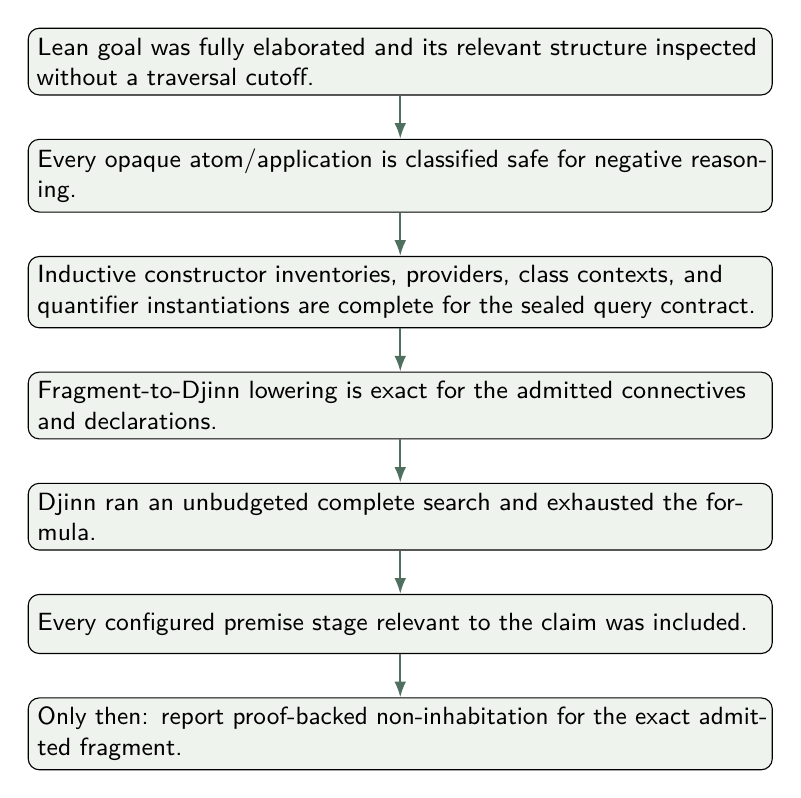
\begin{tikzpicture}[
  node distance=5.5mm,
  check/.style={draw,rounded corners,fill=Panel,align=left,font=\small\sffamily,
    text width=0.76\textwidth,minimum height=7.5mm},
  arr/.style={-{Latex[length=2mm]},thick,color=Sage}]
\node[check] (a) {Lean goal was fully elaborated and its relevant structure inspected without a traversal cutoff.};
\node[check,below=of a] (b) {Every opaque atom/application is classified safe for negative reasoning.};
\node[check,below=of b] (c) {Inductive constructor inventories, providers, class contexts, and quantifier instantiations are complete for the sealed query contract.};
\node[check,below=of c] (d) {Fragment-to-Djinn lowering is exact for the admitted connectives and declarations.};
\node[check,below=of d] (e) {Djinn ran an unbudgeted complete search and exhausted the formula.};
\node[check,below=of e] (f) {Every configured premise stage relevant to the claim was included.};
\node[check,below=of f] (g) {Only then: report proof-backed non-inhabitation for the exact admitted fragment.};
\foreach \x/\y in {a/b,b/c,c/d,d/e,e/f,f/g}\draw[arr] (\x) -- (\y);
\end{tikzpicture}
\end{center}

A single failed link downgrades the wording.

\section{Exact, safe opacity versus unsafe opacity}

Opacity is not automatically fatal.  If a universally quantified abstract formula is sealed as an atom and the structural calculus treats it parametrically, exhaustive failure may still be meaningful.  But an opaque concrete type can hide a constructor or theorem.  For example, treating \term{Nat} as an arbitrary atom and searching for \term{Nat} from no premises would return no proof, although \term{0} is an inhabitant.

Leant's safety bit and completeness facts distinguish these cases.  Concrete constants and fixed applications generally prevent a structural absence from becoming a Lean-level refutation unless their constructor inventory is represented exactly.

\section{Quantifier plans}

Higher-rank and impredicative synthesis may require instantiating polymorphic premises.  A bounded finite plan can discover useful candidates, but failure after finitely many guessed instantiations is not a proof that no instantiation works.

The completeness ledger records whether the current quantifier fragment and plan are among the exact complete cases.  Ambiguous trailing instantiations that are merely rendered as variants also cannot support negative authority.

\section{Provider-relative completeness}

A closed formula may be uninhabited from local assumptions but inhabited using a global provider.  Leant's query contract therefore includes the provider stages and inventories actually searched.

Even a complete provider scan over one live environment would establish only environment-relative absence.  Leant uses bounded query-directed discovery, so most provider-enabled failures remain explicitly inconclusive.

\section{Recursive and instance-related downgrades}

A recursive type with bounded unfolding may hide arbitrarily deep constructor terms.  A hidden instance dictionary may carry methods or data.  A partial constructor inventory may omit a branch.  Each is acceptable for positive search because Lean checks candidates; each blocks strong negative interpretation.

\section{Djinn versus Exference wording}

Djinn can produce an internal evidence value corresponding to proved uninhabitability only when its formula search is complete.  Leant still gates that value through fragment safety.

Exference never grants Leant a refutation.  Even if its queue reports natural exhaustion, the engine is used as a heuristic candidate generator under a finite environment and option set.  Leant reports absence, limits, and pruning diagnostics without calling the Lean type uninhabited.

\begin{keyidea}[A useful three-valued mental model]
For a synthesis query, think in three broad outcomes:
\begin{enumerate}
\item \textbf{verified inhabitant}: a concrete Lean term checked;
\item \textbf{proved uninhabited in the exact admitted contract}: a rare, evidence-backed negative;
\item \textbf{unknown under current translation/search bounds}: the normal meaning of exhaustive-looking failure outside that contract.
\end{enumerate}
\end{keyidea}

\section{Failure transparency}

Good diagnostics report why authority was lost: unsafe opaque atoms, hidden instances, recursive partiality, bounded search, provider limits, rendering rejection, or Lean elaboration errors.  Leant's debug mode can expose the fragment, providers, rendering variants, engine notes, and metrics needed to understand a result.

\begin{sourcebox}
The refutation gate is owned by \url{https://github.com/VladimirReshetnikov/Leant/blob/49c8f9f100a644b5a32b3c942bc6565a3a3ba6a0/src/Leant/Synth/Engine.hs}; fragment safety originates in \path{src/Leant/Synth/Fragment.hs}.  Djinn's budget/exhaustion distinction is in \path{Djinn/Internal/LJT.hs}; Exference's completion states distinguish natural exhaustion, limits, pruning, and identifier exhaustion.
\end{sourcebox}

\begin{recapbox}
A negative result is a theorem about a search contract, not the absence of output.  Leant needs exact translation, safe opacity, complete inventories and premise stages, and unbounded Djinn exhaustion.  Otherwise the correct result is unknown or not found within bounds.
\end{recapbox}

\chapter{The Interactive Layer: \texttt{:synth}, \texttt{:prove}, Sessions, and Debugging}\label{ch:repl}

\section{Expression-oriented interaction}

Leant is designed for rapid exploration.  Users can submit Lean declarations and expressions, inspect types and values, synthesize terms, enter proof workflows, and refer to previous results through \term{it}-style bindings.

The Haskell frontend remembers the Lean environment identifier after each accepted command.  A failed speculative command need not destroy the prior state.  History and snapshots support replay into a fresh backend process when necessary.

\section{\texttt{:synth}}

The synthesis command asks for whole terms inhabiting a goal.  Relevant controls include:

\begin{itemize}
\item engine selection: Djinn, Exference, or both;
\item number of accepted candidates;
\item search steps, queue/depth limits, and alternative policy;
\item provider and library settings;
\item classical fallback;
\item debug output;
\item optional Length assessment.
\end{itemize}

The command is best suited to structurally informative types: adapters, combinators, product/sum rearrangements, polymorphic plumbing, constructor assembly, and applications of known providers.

\section{\texttt{:prove}}

Proof mode works with goals in an interactive Lean proof state.  It can use synthesis to propose a term for a current goal, but it also benefits from ordinary Lean tactics for rewriting, induction, simplification, arithmetic, and dependent case analysis.

This division reflects the theory:

\begin{itemize}
\item \term{:synth} searches for an inhabitant of a comparatively self-contained target;
\item \term{:prove} can transform a difficult dependent goal into simpler structural subgoals before synthesis is invoked.
\end{itemize}

A vector theorem may first require induction and index rewriting; a residual branch might then reduce to a product/function wiring problem that Djinn handles well.

\section{Provider caches and environment identity}

Provider discovery can be expensive.  Leant caches inventories under keys derived from the live environment and query information.  A cache hit is valid only if the exact environment assumptions remain stable.  Replaying a session or changing imports can invalidate provider worlds.

The cache stores checked semantic records, not merely names.  Reusing a string list across environments could associate a name with a different declaration or miss new instances.

\section{Debugging a missing candidate}

When an expected term does not appear, inspect the pipeline in order:

\begin{enumerate}
\item Did the raw goal elaborate as intended?
\item Which subtrees became arrows/products/sums, applications, inductives, or opaque atoms?
\item Was a depth or kind limit reached?
\item Were the needed providers discovered, and under what schemes?
\item Which engine ran, with what bounds?
\item Did the engine produce a semantic candidate?
\item Which Lean variants were rendered?
\item Why did Lean reject them?
\end{enumerate}

This avoids blaming ``search'' for a failure caused by provider discovery or rendering, and avoids blaming ``Lean'' for a candidate never generated.

\section{Reading source ownership}

A useful source map is:

\begin{center}
\begin{tabularx}{\textwidth}{@{}l X@{}}
\toprule
Concern & Primary Leant source \\
\midrule
interactive state and command orchestration & \path{src/Main.hs} \\
Lean process protocol and timeouts & \path{src/Leant/Backend.hs} \\
Lean-side goal/provider serialization & \path{src/Leant/Synth/Fragment.hs} \\
fragment-to-Djex preparation and search & \path{src/Leant/Synth/Engine.hs} \\
Djex-term-to-Lean reconstruction & \path{src/Leant/Synth/Render.hs} \\
lazy group verification & \path{src/Leant/Synth/Verification.hs} \\
semantic provenance invariants & \path{docs/synth-internals.md} \\
user-facing commands and examples & \path{README.md}, \path{docs/Leant.tex} \\
\bottomrule
\end{tabularx}
\end{center}

For Djex, begin with \path{README.md}, then shared \path{synthesis/src/Language/Haskell/Synthesis}, Djinn's \path{Internal/LJT*.hs}, and Exference's \path{Core/Internal/Exference.hs}.

\begin{recapbox}
The REPL layer preserves a live Lean environment and exposes synthesis as one tool among ordinary declarations and proof operations.  Debugging is easiest when the pipeline stages are inspected separately.  Source ownership is intentionally narrow enough that each semantic boundary has a clear home.
\end{recapbox}


\part{Worked Traces and Boundaries}

\chapter{Worked Structural Synthesis Traces}\label{ch:worked-structural}

This chapter follows representative goals through the conceptual pipeline.  The exact debug spelling may evolve, but the semantic stages are fixed by the pinned source.

\section{Composition}

Consider:

\begin{leanblock}[Leant query]
:synth ((A → B → C) → (A → B) → A → C)
\end{leanblock}

\subsection*{Lean elaboration}

With auto-implicit variables, Lean elaborates $A$, $B$, and $C$ as implicit sort variables and the goal as nested $\Pi$-types.  The value binders are non-dependent arrows.

\subsection*{Fragment}

The structural fragment is

\[
(A \to B \to C) \to (A \to B) \to A \to C,
\]

with $A,B,C$ rigid variables.  No opaque atoms, inductives, providers, instances, or bounds are needed.

\subsection*{Djinn formula and proof search}

The formula is the same propositional implication shape.  Right rules introduce $f$, $g$, and $x$.  The atomic goal is $C$.

The context contains:

\[
f:A\to B\to C,
\qquad g:A\to B,
\qquad x:A.
\]

To use $f$, search must provide $A$ and $B$.  It uses $x$ for $A$ and applies $g$ to $x$ for $B$.  The proof term is equivalent to

\[
\lambda f.\lambda g.\lambda x.\,f\,x\,(g\,x).
\]

\subsection*{Rendering and verification}

The renderer chooses fresh Lean binder names and emits:

\begin{leanblock}[Candidate]
fun f g x => f x (g x)
\end{leanblock}

Lean checks it against the exact original goal.  Because the fragment was exact and Djinn's unbudgeted search is complete, failure could also have had a strong logical interpretation; in this case a verified positive answer ends the story.

\section{Swapping a product}

For data:

\begin{leanblock}[Product swap]
:synth (A × B → B × A)
\end{leanblock}

or for propositions:

\begin{leanblock}[Conjunction swap]
:synth (P ∧ Q → Q ∧ P)
\end{leanblock}

both lower to a product-swap shape.  The exact nominal families and result sort are retained outside the formula calculus.  Djinn's proof term splits the input pair and constructs a pair in reverse order.

The renderer can use expected-type syntax:

\begin{leanblock}[Universe-agnostic product syntax]
fun p => ⟨p.2, p.1⟩
\end{leanblock}

Lean resolves the appropriate constructor and projections from the expected type.  Search shares a logical shape; verification restores the actual Lean family.

\section{Sum reassociation}

Consider:

\begin{leanblock}[A sum transformation]
:synth (A ⊕ (B ⊕ C) → (A ⊕ B) ⊕ C)
\end{leanblock}

The formula becomes a constructor-tagged disjunction.  A proof must case-analyze the input:

\begin{leanblock}[Representative candidate]
fun s =>
  match s with
  | .inl a => .inl (.inl a)
  | .inr (.inl b) => .inl (.inr b)
  | .inr (.inr c) => .inr c
\end{leanblock}

The exact syntax may use qualified constructors depending on context, but the semantic proof contains three branches and tagged injections.  Constructor descriptors preserved during lowering prevent the branches of unrelated sum-like inductives from being confused.

\section{A local continuation pattern}

The type

\begin{leanblock}[Continuation-shaped structural goal]
((A → B) → A) → (A → B) → B
\end{leanblock}

is not intuitionistically inhabited in general: from $k:(A\to B)\to A$ and $f:A\to B$, one can derive $k\,f:A$ and then $f(k\,f):B$.  In fact it \emph{is} inhabited, and Djinn can discover:

\begin{leanblock}[Candidate]
fun k f => f (k f)
\end{leanblock}

The example illustrates why visual intuition can be unreliable.  Systematic proof search explores how assumptions' result atoms can feed one another.

\begin{recapbox}
For exact arrows, products, and sums, the pipeline closely follows Curry--Howard introduction and elimination rules.  Lean-specific nominal details ride alongside the formula and return during rendering.  Verification confirms that the reconstructed syntax matches the original family and binder structure.
\end{recapbox}

\chapter{A Complete Negative Trace}\label{ch:worked-negative}

\section{The target}

Consider the polymorphic type:

\begin{leanblock}[Leant query]
:synth (∀ A B : Type, A → B)
\end{leanblock}

No assumptions, axioms, bottom values, unsafe operations, or providers are present in the closed goal.

\section{Rigid quantification}

Lean elaborates $A$ and $B$ as explicit type binders.  Leant admits them as rigid universally quantified type variables.  Rigid means that search cannot unify $A$ with $B$ merely to make the arrow look like identity.

The body is $A\to B$.  Right introduction gives a hypothetical $x:A$ and leaves atomic goal $B$.

\section{Exhaustive LJT failure}

The context contains only $x:A$.  There is:

\begin{itemize}
\item no hypothesis of type $B$;
\item no implication ending in $B$;
\item no product or sum whose elimination yields $B$;
\item no constructor inventory or provider for arbitrary rigid $B$;
\item no falsity from which to eliminate.
\end{itemize}

The LJT search space closes without a proof.

\section{Why this failure can be conclusive}

For this goal, the relevant ledger can be exact:

\begin{itemize}
\item only sort quantification and one ordinary arrow occur;
\item the variables are abstract and rigid;
\item no concrete opaque atom conceals an inhabitant;
\item no indexed or recursive inductive is involved;
\item no instance binder or provider stage is needed;
\item Djinn can run unbudgeted.
\end{itemize}

Leant can therefore report proof-backed uninhabitation for the admitted constructive fragment, rather than merely ``no term found.''

\section{What would change the conclusion}

Adding any of the following changes the problem:

\begin{leanblock}[Extra premises that make the target inhabitable]
-- A direct provider:
(∀ A B : Type, (A → B) → A → B)

-- Falsity in the context:
False → (∀ A B : Type, A → B)

-- Classical choice plus a nonempty assumption for B:
∀ A B : Type, Nonempty B → A → B
\end{leanblock}

The first returns the supplied function.  The second eliminates falsity.  The third may choose a $B$ from nonemptiness under suitable classical principles.  Refutation is always relative to the exact context.

\begin{warningbox}[Do not confuse parametric impossibility with runtime tricks]
A partial language could implement \term{A → B} by looping forever or throwing an unchecked exception.  Lean's safe logical fragment requires total terms.  Unsafe or partial executable definitions do not become proofs of arbitrary propositions.
\end{warningbox}

\begin{recapbox}
The negative result works because the type translates exactly, universal variables stay rigid, no hidden structure or premise exists, and complete LJT search exhausts.  This is the model case for Leant's strongest negative wording.
\end{recapbox}

\chapter{Dependent Cargo: What Works Without Dependent Search}\label{ch:worked-cargo}

\section{Moving an opaque dependent formula}

Declare:

\begin{leanblock}[Dependent propositions]
opaque P : Nat → Prop
opaque Q : Prop
\end{leanblock}

and ask for:

\begin{leanblock}[Structural use of dependency]
:synth (((∀ n : Nat, P n) ∧ Q) →
        (Q ∧ (∀ n : Nat, P n)))
\end{leanblock}

Let

\[
X = \forall n:\mathsf{Nat},\,P(n).
\]

Leant seals the entire $X$ as one alpha-aware atom.  The formula seen by Djinn is $(X\land Q)\to(Q\land X)$.  A product-swap proof is sufficient.

A representative Lean term is:

\begin{leanblock}[Candidate]
fun h => ⟨h.2, h.1⟩
\end{leanblock}

The term never inspects the proof of $X$.  It merely returns the same proof object in another field.  Lean's expected type confirms that \term{h.1} has the exact dependent proposition.

\section{Instantiating the dependent premise does not work by mere opacity}

Now ask for:

\begin{leanblock}[Requires dependent application]
(∀ n : Nat, P n) → P 0
\end{leanblock}

The obvious term is:

\begin{leanblock}[Human-written term]
fun h => h 0
\end{leanblock}

But if the premise \term{∀ n, P n} is sealed as one atom $X$ and the goal \term{P 0} as another atom $Y$, the propositional formula is $X\to Y$.  No relationship between $X$ and $Y$ is visible.  Moving opaque cargo is sound; opening it to perform dependent application requires a richer rule.

Leant has bounded support for selected quantified type instantiations, especially Haskell-like sort polymorphism.  A value-indexed dependent forall over \term{Nat} is a different feature and should not be inferred from that support.

\section{Transport is likewise invisible}

Consider:

\begin{leanblock}[Transport target]
∀ (α : Type) (n m : Nat),
  n = m → Vector α n → Vector α m
\end{leanblock}

A human can write:

\begin{leanblock}[Human-written transport]
fun α n m h v => h ▸ v
\end{leanblock}

The essential step eliminates equality into a type family.  A propositional search that treats \term{n = m}, \term{Vector α n}, and \term{Vector α m} as unrelated atoms cannot synthesize it.  Erasing the indices would be unsound; preserving them opaquely is safe but incomplete.

\section{Use proof mode to expose structural subgoals}

In a larger theorem, ordinary Lean tactics can perform induction or rewriting first.  After substituting $m$ for $n$, the remaining vector term may have exactly the expected type by definitional equality.  If the residual goal is a function/product/sum wiring problem, synthesis can then help.

This is the intended collaboration:

\begin{center}
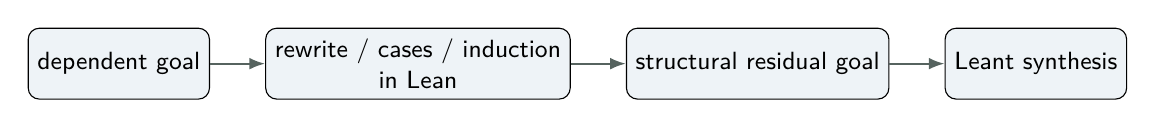
\begin{tikzpicture}[
  node distance=7mm,
  box/.style={draw,rounded corners,fill=PanelBlue,font=\small\sffamily,align=center,minimum height=9mm},
  arr/.style={-{Latex[length=2mm]},thick,color=MutedInk}]
\node[box] (dep) {dependent goal};
\node[box,right=of dep] (tac) {rewrite / cases / induction\\in Lean};
\node[box,right=of tac] (str) {structural residual goal};
\node[box,right=of str] (syn) {Leant synthesis};
\draw[arr] (dep)--(tac);
\draw[arr] (tac)--(str);
\draw[arr] (str)--(syn);
\end{tikzpicture}
\end{center}

\begin{keyidea}[A precise capability statement]
Leant can often \emph{transport values whose types are dependent} through surrounding structural logic.  It generally cannot \emph{reason inside those dependent types} by inventing indices, motives, equality proofs, or transports.
\end{keyidea}

\begin{recapbox}
Opaque cargo supports rearrangement, storage, and application through already exposed premises.  It does not reveal dependent elimination rules.  Value-indexed foralls, equality transport, and indexed pattern matching remain jobs for Lean tactics or a future richer synthesis calculus.
\end{recapbox}

\chapter{Polymorphism, Rank-N Use, and Rendering Variants}\label{ch:worked-rankn}

\section{A polymorphic argument}

Consider:

\begin{leanblock}[Rank-N target]
((∀ α : Type, α → α) → Nat)
\end{leanblock}

The argument $f$ is itself polymorphic.  One inhabitant is:

\begin{leanblock}[Candidate]
fun f => f Nat 0
\end{leanblock}

The type variable $\alpha$ is nested inside the domain of the outer function, so this is higher-rank use.  Search must instantiate $f$ at \term{Nat} and then provide \term{0}.

\section{How the type crosses the boundary}

Leant classifies the outer binder as a value arrow.  The domain retains an explicit \term{ForallType} over a rigid type variable, with body $\alpha\to\alpha$.  Djex's higher-rank machinery and rigid instantiation plan may expose an application of $f$ at an admitted ground type.

The natural-number result requires a constructor or provider.  With the recursive \term{Nat} declaration represented sufficiently for positive introduction, zero is available.  Positive success is safe even if recursive completeness is bounded, because Lean verifies the concrete term.

\section{Why a renderer may need variants}

The original binder \term{∀ α : Type, ...} is explicit.  A source scheme written with braces would be implicit:

\begin{leanblock}[Implicit polymorphic argument]
({α : Type} → α → α) → Nat
\end{leanblock}

Depending on the exact source binder, a candidate application might need \term{f Nat 0}, \term{f 0}, or \term{f (α := Nat) 0}.  The engine's abstract application does not by itself encode every surface choice.  Leant's side metadata and bounded variant enumerator reconstruct candidates and let Lean choose the valid one.

\section{Ambiguity weakens negative evidence}

If positive search finds a semantic application but every reconstruction variant fails, no verified candidate is shown.  Conversely, a bounded instantiation plan that finds no semantic application does not prove none exists.  Higher-rank positive support and higher-rank complete refutation are different capabilities.

\begin{recapbox}
Djex's source language can represent selected higher-rank type schemes even though it is not dependently typed.  Leant records binder visibility and may enumerate application spellings.  Positive candidates are verified; bounded instantiation and reconstruction prevent broad negative conclusions.
\end{recapbox}

\chapter{Provider-Guided and Library-Guided Synthesis}\label{ch:worked-provider}

\section{A global conversion function}

Imagine a live Lean environment containing:

\begin{leanblock}[Environment declarations]
opaque A : Type
opaque B : Type
opaque convert : A → B
\end{leanblock}

A query for \term{A → B} has no closed structural inhabitant if $A$ and $B$ are unrelated atoms.  If provider discovery admits \term{convert}, the search environment gains a premise of exactly that type.  Djinn or Exference can produce:

\begin{leanblock}[Provider-backed candidate]
fun x => convert x
\end{leanblock}

The candidate's origin records that \term{convert} was a live provider, not a local lambda binder.  The renderer restores its exact global name; Lean resolves the declaration in the current environment and checks the application.

\section{Polymorphic providers}

Suppose:

\begin{leanblock}[A polymorphic provider]
opaque mapBox {α β : Type} : (α → β) → Box α → Box β
\end{leanblock}

For a goal \term{(A → B) → Box A → Box B}, provider matching must instantiate $\alpha:=A$ and $\beta:=B$.  The exact type-constructor applications \term{Box A} and \term{Box B} must retain both nominal head and arguments; flattening them to unrelated text or a single \term{Box} atom would break unification.

A renderer may emit:

\begin{leanblock}[Provider application]
fun f x => mapBox f x
\end{leanblock}

and let Lean infer the implicit type arguments.

\section{Class-constrained providers}

A provider might require \term{[C α]}.  Lean's provider scanner can ask the live instance resolver for complete assignments and preserve structured exact context metadata.  If a valid assignment exists, a rendered term may leave the dictionary implicit.

Failure to find one within the bounded scan does not prove the provider unusable in every possible elaboration context.  The completeness ledger records that limitation.

\section{Library recursion as a provider}

Suppose a user wants a list transformation that can be expressed by an existing combinator such as \term{List.map}, \term{List.foldr}, or a curated recursor.  Library mode can make the combinator a premise.  Search then synthesizes its arguments rather than inventing recursion.

This decomposition is powerful:

\[
\text{recursive algorithm invention}
\quad\Longrightarrow\quad
\text{application synthesis over a trusted recursive combinator}.
\]

The final term remains ordinary Lean code, and its provider use is checked.

\section{Why results depend on configuration}

Provider and library settings change the search environment, so they change both positive candidates and the meaning of failure.  A query that is uninhabited in pure intuitionistic structure may become inhabited after enabling a provider, a classical theorem, or a recursor.

A reproducible synthesis report should therefore include:

\begin{itemize}
\item Lean environment/import state;
\item provider and library modes;
\item engine and resource settings;
\item quantifier/recursive policies;
\item exact verified candidate.
\end{itemize}

\begin{recapbox}
Providers bridge imported Lean functionality into the search calculus.  Exact names, schemes, type applications, constraints, and environment identity are preserved.  Curated recursion converts hard recursive invention into ordinary combinator application.  Configuration is part of the query contract.
\end{recapbox}

\chapter{The Optional Length/Z3 Behavioral Layer}\label{ch:length}

\section{Why types are not enough}

For \term{List α → List α}, structural synthesis may return several verified terms.  Suppose the user additionally wants output length to equal input length.  That property is not encoded in the type, so ordinary Lean verification cannot distinguish identity from constant-empty.

Djex contains an experimental semantic Length layer for a narrowly defined class of list-spine and product problems.  Leant can optionally use it to assess already type-correct Exference candidates.

\section{The authority order}

The order is essential:

\begin{enumerate}
\item synthesize a candidate through the ordinary engine;
\item render and verify it against the exact Lean type;
\item retain its exact typed candidate graph and inventory sidecar;
\item seal a supported Length contract and target;
\item symbolically interpret the graph under an explicit provider-law basis;
\item encode the resulting bounded arithmetic problem as canonical QF\_LIA SMT-LIB;
\item run Z3 through a resource-bounded process/session boundary;
\item independently replay any model or claimed bounded-positive result against the original checked semantic problem;
\item issue only the narrow receipt or ranking decision authorized by that replay.
\end{enumerate}

Z3 never makes an ill-typed term well typed.  Lean verification happened first.  Conversely, Lean type verification does not prove the Length postcondition; that is a separate, explicitly bounded semantic claim.

\section{Sealed contracts and typed graphs}

The behavioral layer does not reparse the rendered Lean string.  It consumes an engine-owned typed term graph tied to:

\begin{itemize}
\item the exact synthesis session and inventory;
\item provider semantics admitted for Length interpretation;
\item the normalized target type and contract;
\item the candidate graph fingerprint;
\item resource and domain policies.
\end{itemize}

This prevents a textually identical term from inheriting a receipt produced under another inventory or contract.

\section{Symbolic length interpretation}

Supported term-graph nodes are interpreted as arithmetic expressions over input lengths.  A provider such as identity may have law $\ell_{out}=\ell_{in}$; constant empty has $\ell_{out}=0$; append has $\ell_{out}=\ell_1+\ell_2$ under a sealed provider law.

Unsupported nodes fail closed.  The interpreter does not guess semantics from function names.  Provider laws belong to the checked session inventory.

\section{SMT solving and replay}

The arithmetic problem is encoded in quantifier-free linear integer arithmetic.  A satisfiable counterexample query may produce concrete natural input lengths violating the postcondition.  Djex re-evaluates those inputs through its own checked semantic problem before returning a validated counterexample.

An unsatisfiable solver response is not automatically a proof.  Bounded-positive receipts require the exact applicable domain and replay policy recorded by the current API.  The semantic documentation repeatedly emphasizes that raw solver status, bytes, or cached samples grant no independent authority.

\section{What the layer can and cannot say}

It can help rank or filter candidates under a supported length contract and bounded domain.  It cannot by itself establish:

\begin{itemize}
\item extensional equality of arbitrary Lean functions;
\item element preservation or permutation;
\item correctness outside the sealed domain;
\item semantics of unsupported providers;
\item a kernel theorem unless a separate proof-producing bridge is built.
\end{itemize}

\begin{keyidea}[Behavioral checks are orthogonal to type checking]
A candidate may be type-correct and behaviorally rejected; another may be behaviorally acceptable under a bounded contract but still rely on axioms or providers the user dislikes.  Leant keeps these judgments separate so the user can see which property was established by which mechanism.
\end{keyidea}

\begin{sourcebox}
The current semantic-origin and Length boundary is summarized in Leant's \path{docs/synth-internals.md}.  The Djex guide and semantic foundations at the pinned submodule revision describe typed candidates, sealed contracts, QF\_LIA queries, bounded Z3 sessions, and independent replay.  The standalone Djex main revision contains later refinements that should not be attributed to Leant until its submodule advances.
\end{sourcebox}

\begin{recapbox}
The Length layer is post-type-check behavioral analysis over sealed typed candidates.  It uses Z3 as a bounded reasoning component and independently replays results.  Its receipts have narrow contract-specific authority and are not Lean proofs of general program correctness.
\end{recapbox}

\chapter{A Reliable Mental Model for Using and Extending Leant}\label{ch:mental-model}

\section{Ask four questions about every result}

When Leant shows a candidate or a failure, ask:

\begin{enumerate}
\item \textbf{What did Lean elaborate?}  Surface notation and auto-implicit variables may hide the exact goal.
\item \textbf{What did the fragment expose?}  Which pieces became logic, applications, inductives, providers, or opaque atoms?
\item \textbf{What did the engine prove or search?}  Djinn formula proof, Exference bounded candidate, or both?
\item \textbf{What did the final checker authorize?}  Lean type acceptance, negative completeness evidence, or a separate behavioral receipt?
\end{enumerate}

These questions prevent most category errors.

\section{Classify goals before searching}

A useful manual classification is:

\begin{description}
\item[Pure structural] Arrows, products, sums, polymorphic plumbing.  Excellent \term{:synth} targets.
\item[Provider structural] Requires a known library function but little semantic reasoning.  Enable provider/library search.
\item[Opaque dependent cargo] Dependent formulas are only moved or stored.  Often works.
\item[Dependent elimination] Requires instantiation at a value, indexed cases, transport, or a motive.  Use Lean tactics/proof mode; synthesis may help later.
\item[Recursive invention] Requires choosing a recursion scheme and branch behavior.  Prefer curated combinators or explicit design.
\item[Behaviorally underdetermined] Many inhabitants share the type.  Add a theorem, refinement, examples, or a supported semantic contract.
\end{description}

\section{Extend at the correct layer}

New functionality belongs in different places depending on its semantic role:

\begin{itemize}
\item recognize another exact Lean connective: serializer/fragment policy;
\item support another Haskell-like type form: Djex shared source representation and both engine adapters;
\item add a proof-search rule: Djinn calculus, proof terms, and proof checker;
\item add a heuristic expression form: Exference nodes, unification, checking, and ranking;
\item reconstruct a known engine term in Lean: renderer plus verification tests;
\item strengthen negative claims: completeness ledger and exactness proof, not only more search;
\item add a behavioral property: typed graph semantics, sealed contract, solver/certificate/replay boundary;
\item support general dependent synthesis: a new calculus and term representation, not an extra opaque-atom case.
\end{itemize}

\section{Prefer fail-closed boundaries}

At every translation, ask what happens when metadata is missing or a bound is exceeded.  The robust answer is usually:

\begin{itemize}
\item keep the subtree opaque for positive transport;
\item mark negative evidence unsafe or incomplete;
\item reject malformed protocol data;
\item drop an unrenderable candidate;
\item let Lean reject ambiguous syntax;
\item report bounded failure as unknown;
\item refuse unsupported behavioral interpretation.
\end{itemize}

This style may miss answers, but it prevents an optimization or convenience path from acquiring proof authority accidentally.

\section{The compact architectural picture}

\begin{center}
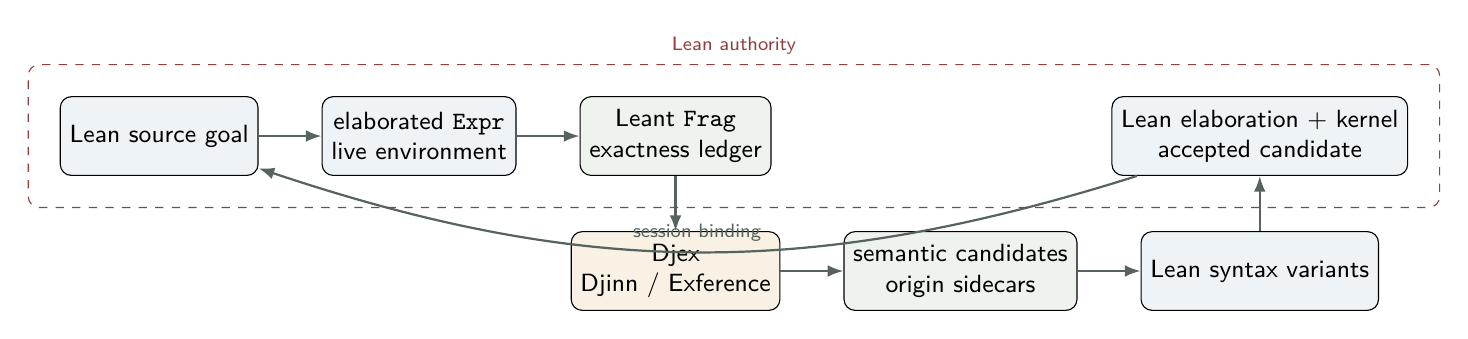
\begin{tikzpicture}[
  node distance=7mm and 8mm,
  box/.style={draw,rounded corners,align=center,font=\small\sffamily,minimum height=10mm},
  arr/.style={-{Latex[length=2mm]},thick,color=MutedInk},
  trust/.style={draw=Red,dashed,rounded corners,inner sep=4mm}]
\node[box,fill=PanelBlue] (goal) {Lean source goal};
\node[box,fill=PanelBlue,right=of goal] (expr) {elaborated \term{Expr}\\live environment};
\node[box,fill=Panel,right=of expr] (frag) {Leant \term{Frag}\\exactness ledger};
\node[box,fill=PanelGold,below=of frag] (djex) {Djex\\Djinn / Exference};
\node[box,fill=Panel,right=of djex] (cand) {semantic candidates\\origin sidecars};
\node[box,fill=PanelBlue,right=of cand] (text) {Lean syntax variants};
\node[box,fill=PanelBlue,above=of text] (verify) {Lean elaboration + kernel\\accepted candidate};
\draw[arr] (goal)--(expr);
\draw[arr] (expr)--(frag);
\draw[arr] (frag)--(djex);
\draw[arr] (djex)--(cand);
\draw[arr] (cand)--(text);
\draw[arr] (text)--(verify);
\draw[arr,bend left=18] (verify) to node[above,font=\scriptsize\sffamily]{session binding} (goal);
\node[trust,fit=(goal)(expr)(verify),label={[font=\scriptsize\sffamily\color{Red}]above:Lean authority}] {};
\end{tikzpicture}
\end{center}

The dashed region is not saying the entire Lean implementation is formally verified.  It indicates where the final type-authority operation occurs.  Djex and the Haskell controller are outside that authority and are made safe for positive answers by the return path through Lean.

\begin{recapbox}
Classify the goal, inspect the fragment, distinguish engine contracts, and identify the final authority.  Extend the layer that owns the missing semantics.  Preserve fail-closed behavior when exactness cannot be established.  This mental model is sufficient to navigate both the codebase and user-facing results.
\end{recapbox}


\chapter*{Conclusion}
\addcontentsline{toc}{chapter}{Conclusion}

Lean's apparent complexity comes from one coherent decision: the type language is expressive enough for types to mention values, propositions to be types, and proofs to be programs.  The Calculus of Constructions supplies the dependent function core; inductive families supply data, recursion, equality, and induction; universes and termination keep the system consistent; elaboration lets humans write concise source; the kernel reduces the result to a small checked expression language.

Leant becomes straightforward once that stack is visible.  It does not replace Lean's type theory with Djex.  It asks Lean to project a goal into an explicitly smaller structural language.  Djinn can decide an exact intuitionistic fragment; Exference can search more flexibly under resource bounds.  Unsupported dependent structure is retained as opaque cargo, not erased.  Candidate terms return through a renderer that is allowed to be wrong because Lean checks every answer.  Negative claims are rarer because they need a complete translation and search ledger.  Optional behavioral analysis remains a separate, sealed judgment.

That architecture yields a useful division of labor:

\begin{center}
\begin{tabularx}{0.92\textwidth}{@{}l X@{}}
\toprule
Component & Responsibility \\
\midrule
Lean elaborator & interpret concise source in the exact live environment \\
Lean kernel & authorize typing, universes, conversion, inductives, and safety \\
Leant fragment & state what structure is exposed and what completeness is lost \\
Djinn & construct or refute proofs in an exact propositional calculus \\
Exference & search ranked typed expressions under explicit limits \\
Leant renderer & reconstruct candidate Lean syntax and bounded variants \\
Verification loop & return every positive answer to Lean \\
Behavioral layer & assess a separate sealed property without borrowing type authority \\
\bottomrule
\end{tabularx}
\end{center}

The shortest durable summary is therefore:

\begin{keyidea}[Rich source, restricted search, authoritative return]
Leant is useful not because Djex understands all of Lean, but because Leant knows exactly when it does not, preserves that boundary as data, and sends every proposed inhabitant back to Lean.
\end{keyidea}

\appendix

\chapter{Lean Syntax and Logic Cheat Sheet}\label{app:syntax}

\section{Declarations}

\begin{longtable}{@{}>{\ttfamily}p{0.29\textwidth} >{\raggedright\arraybackslash}p{0.65\textwidth}@{}}
\toprule
\normalfont Form & \normalfont Meaning \\
\midrule
\endfirsthead
\toprule
\normalfont Form & \normalfont Meaning \\
\midrule
\endhead
def f (x : A) : B := t & transparent named definition checked at type $B$ \\
theorem h : P := p & opaque checked proof of proposition $P$ \\
example : T := t & check a temporary unnamed declaration \\
opaque c : T & introduce a checked opaque constant (with a body in full form) \\
axiom a : T & assume a constant of type $T$ without a body \\
inductive I ... where ... & declare an inductive family and constructors \\
structure S ... where ... & one-constructor inductive with named fields \\
class C ... where ... & structure designated for instance search \\
instance : C A := ... & register a term for type-class resolution \\
namespace N ... end N & qualify enclosed names \\
open N & make namespace members available for resolution/printing \\
import M & load a compiled module and its environment declarations \\
\bottomrule
\end{longtable}

\section{Binders}

\begin{center}
\begin{tabularx}{\textwidth}{@{}l l X@{}}
\toprule
Syntax & Kind & Caller behavior \\
\midrule
\term{(x : A)} & explicit & normally supplied \\
\term{{x : A}} & implicit & normally inferred \\
\term{{{x : A}}} & strict implicit & inferred when later explicit use triggers insertion \\
\term{[x : C]} & instance implicit & synthesized by type-class resolution \\
\term{∀ x : A, B x} & dependent binder & proposition/function according to codomain sort \\
\bottomrule
\end{tabularx}
\end{center}

\section{Term forms}

\begin{longtable}{@{}>{\ttfamily}p{0.34\textwidth} >{\raggedright\arraybackslash}p{0.60\textwidth}@{}}
\toprule
\normalfont Syntax & \normalfont Reading \\
\midrule
\endfirsthead
\toprule
\normalfont Syntax & \normalfont Reading \\
\midrule
\endhead
fun x => t & lambda abstraction \\
f x y & left-associated application \\
A → B → C & right-associated function type \\
let x := a; t & local definition \\
match s with | ... & pattern matching, elaborated to recursors \\
⟨a, b⟩ & anonymous constructor selected by expected type \\
p.1, p.2, p.field & projections \\
\term{_} & elaboration metavariable / placeholder \\
@f & expose normally implicit arguments of $f$ at the surface \\
f (α := A) & named explicit assignment to an implicit parameter \\
by ... & tactic script constructing a term \\
rfl & reflexivity term/tactic, succeeds up to definitional equality \\
h ▸ x & transport/rewrite $x$ along equality $h$ \\
\bottomrule
\end{longtable}

\section{Logical forms}

\begin{center}
\begin{tabularx}{\textwidth}{@{}l X X@{}}
\toprule
Lean & Constructor/eliminator intuition & Search shape \\
\midrule
\term{P → Q} & lambda / application & implication \\
\term{P ∧ Q} & pair / projections & conjunction \\
\term{P ∨ Q} & injection / cases & disjunction \\
\term{True} & unique constructor & top \\
\term{False} & no constructor / eliminate anywhere & bottom \\
\term{¬ P} & function $P\to\mathsf{False}$ & implication to bottom \\
\term{∀ x : A, P x} & dependent lambda/application & full dependency; only selected fragments exposed \\
\term{∃ x : A, P x} & witness + proof / dependent cases & dependent inductive in \term{Prop} \\
\term{x = y} & \term{Eq.refl} / transport & indexed inductive \\
\bottomrule
\end{tabularx}
\end{center}

\section{Inspection commands useful around Leant}

\begin{longtable}{@{}>{\ttfamily\small\raggedright\arraybackslash}p{0.45\textwidth} >{\raggedright\arraybackslash}p{0.49\textwidth}@{}}
\toprule
\normalfont Command & \normalfont Purpose \\
\midrule
\endfirsthead
\toprule
\normalfont Command & \normalfont Purpose \\
\midrule
\endhead
\#check t & elaborate $t$ and print its type \\
\#eval t & compile/evaluate a computable expression \\
\#reduce t & reduce an expression through the elaborator/kernel reduction facilities \\
\#print name & print a declaration \\
\#print axioms name & report axiomatic dependencies \\
\term{set_option pp.all true} & expose more elaborated detail in pretty printing \\
\term{set_option trace.Meta.synthInstance true} & inspect type-class search (version/options permitting) \\
\bottomrule
\end{longtable}

\chapter{Compact Formal Rules}\label{app:rules}

This appendix collects a schematic core sufficient to decode the theoretical discussion.  It is not a complete formal specification of Lean's kernel, inductive checker, quotient primitives, safety classes, or optimized conversion algorithm.

\section{Contexts and sorts}

\begin{formalbox}[Context extension]
\[
\frac{\Gamma\ \mathsf{ctx}\qquad \Gamma\vdash A:\mathsf{Sort}\;u\qquad x\notin\Gamma}
     {\Gamma,x:A\ \mathsf{ctx}}
\]
\end{formalbox}

\begin{formalbox}[Sort formation]
\[
\Gamma\vdash \mathsf{Sort}\;u : \mathsf{Sort}(u+1).
\]
\end{formalbox}

Lean additionally validates that every named universe parameter is declared and that no level metavariable reaches the kernel.

\section{Dependent products}

\begin{formalbox}[$\Pi$ formation]
\[
\frac{\Gamma\vdash A:\mathsf{Sort}\;u
      \qquad
      \Gamma,x:A\vdash B:\mathsf{Sort}\;v}
     {\Gamma\vdash \Pi(x:A),B:\mathsf{Sort}(\operatorname{imax}(u,v))}
\]
\end{formalbox}

\begin{formalbox}[Lambda]
\[
\frac{\Gamma,x:A\vdash t:B}
     {\Gamma\vdash \lambda(x:A),t : \Pi(x:A),B}
\]
\end{formalbox}

\begin{formalbox}[Application]
\[
\frac{\Gamma\vdash f:\Pi(x:A),B
      \qquad
      \Gamma\vdash a:A}
     {\Gamma\vdash f\,a:B[a/x]}
\]
\end{formalbox}

\section{Local definitions}

\begin{formalbox}[Let]
\[
\frac{\Gamma\vdash A:\mathsf{Sort}\;u
      \qquad
      \Gamma\vdash a:A
      \qquad
      \Gamma,x:A\vdash t:B}
     {\Gamma\vdash (\mathsf{let}\;x:A:=a;\,t):B[a/x]}
\]
\end{formalbox}

Zeta reduction makes the let expression definitionally equal to $t[a/x]$.

\section{Conversion}

\begin{formalbox}[Definitional conversion]
\[
\frac{\Gamma\vdash t:A
      \qquad A\defeq B
      \qquad \Gamma\vdash B:\mathsf{Sort}\;u}
     {\Gamma\vdash t:B}
\]
\end{formalbox}

Lean's implemented $\defeq$ includes reduction and congruence, proof irrelevance, function eta expansion, eta for suitable nonrecursive structures, literal reduction, and environment-guided lazy unfolding.

\section{Dependent pairs}

A schematic $\Sigma$ rule is:

\begin{formalbox}[$\Sigma$ introduction]
\[
\frac{\Gamma\vdash a:A\qquad \Gamma\vdash b:B[a/x]}
     {\Gamma\vdash \langle a,b\rangle : \Sigma(x:A),B}
\]
\end{formalbox}

Lean implements \term{Sigma} as an inductive family rather than a primitive \term{Expr} constructor.  Its eliminator is therefore generated by the inductive machinery.

\section{Equality elimination}

A schematic dependent eliminator is:

\[
\mathsf{Eq.rec} :
\Pi\{\alpha:\mathsf{Sort}\;u\}\{a:\alpha\}
(P:\Pi b:\alpha, a=b\to\mathsf{Sort}\;v),
P\;a\;\mathsf{rfl}\to
\Pi\{b:\alpha\}(h:a=b),P\;b\;h.
\]

Simpler transport is derived by choosing a motive that ignores the equality proof.  Pattern matching and rewriting elaborate to applications of such eliminators.

\section{Inductive declarations}

A full rule must check at least:

\begin{itemize}
\item constructor types are well formed in declared universes;
\item constructor results target the declared inductive family with correct parameters;
\item recursive occurrences satisfy positivity;
\item universe and elimination constraints are respected;
\item mutual blocks are coherent;
\item generated recursors type check.
\end{itemize}

Lean's kernel compiles the accepted block into ordinary constants and recursors.  User pattern matching is then elaborated to those constants.

\chapter{Lean-to-Leant Translation Reference}\label{app:mapping}

\begin{longtable}{@{}>{\raggedright\arraybackslash}p{0.25\textwidth} >{\raggedright\arraybackslash}p{0.24\textwidth} >{\raggedright\arraybackslash}p{0.43\textwidth}@{}}
\toprule
Lean shape & Leant/Djex treatment & Consequence \\
\midrule
\endfirsthead
\toprule
Lean shape & Leant/Djex treatment & Consequence \\
\midrule
\endhead
non-dependent $A\to B$ & \term{FArr}, then function/implication & fully structural when children exact \\
\term{And P Q} & product/conjunction plus nominal restoration & Djinn splits/builds pair \\
\term{Prod A B}, \term{PProd A B} & Lean product fragment plus nominal restoration & same logical search shape, exact expected-type check \\
\term{Or P Q}, \term{Sum A B}, \term{PSum A B} & tagged sum & injections and case analysis \\
\term{Iff P Q} & pair of implications & exact logical expansion \\
\term{Not P} & $P\to\bot$ & exact definitional/logical expansion \\
true/unit families & top/unit & immediate constructor \\
false/empty families & nominal bottom & no introduction; elimination if premise exists \\
sort-bound forall & \term{FAll}, rigid Djex forall & selected polymorphism and bounded rank-N use \\
non-dependent value forall & arrow & ordinary lambda/application \\
value-dependent forall & opaque atom unless dedicated case & can be moved; not generally instantiated \\
instance-implicit forall & \term{FInst} or exact provider context & positive elaboration possible; negative evidence guarded \\
type-valued nominal application & \term{FApp} retaining head and args & higher-kinded unification/provider matching \\
term-indexed application & opaque identity & no index-sensitive reasoning \\
complete nonrecursive nonindexed inductive & constructor-tagged sum of products & construction and case analysis \\
indexed inductive & opaque & no dependent constructor refinement \\
constructor with dependent field & opaque & no dependent pair elimination \\
recursive inductive & bounded recursive fragment & limited positive support; completeness guarded \\
incomplete declaration inventory & partial fragment/opaque downgrade & positive candidates checked; no strong negative \\
traversal fuel exhausted & depth marker/completeness downgrade & failure means unknown \\
concrete unsupported constant & unsafe opaque atom for refutation & may hide a known inhabitant \\
abstract universally quantified subtree & possibly refutation-safe opaque atom & parametric structural reasoning may remain complete \\
\bottomrule
\end{longtable}

\chapter{Interpreting Leant Outcomes}\label{app:outcomes}

\begin{longtable}{@{}>{\raggedright\arraybackslash}p{0.28\textwidth} >{\raggedright\arraybackslash}p{0.30\textwidth} >{\raggedright\arraybackslash}p{0.34\textwidth}@{}}
\toprule
Observed outcome & What is authorized & What is not authorized \\
\midrule
\endfirsthead
\toprule
Observed outcome & What is authorized & What is not authorized \\
\midrule
\endhead
Lean-verified candidate & the displayed term inhabits the exact goal in the live environment & intended behavior, efficiency, uniqueness, completeness \\
Djinn proof before Lean verification & a proof term exists in the translated formula calculus & valid Lean syntax or exact Lean typing \\
all render variants rejected & this reconstruction route produced no accepted term & source type uninhabited \\
Exference step limit & no candidate in explored prefix & search exhaustion or uninhabitation \\
Exference natural exhaustion & no candidate in sealed finite Exference search state & general Lean uninhabitation \\
Djinn budget exhausted & no proof in explored choice prefix & formula unprovable \\
unbounded Djinn formula exhaustion & translated exact formula unprovable & Lean goal uninhabited unless completeness ledger also passes \\
proof-backed Leant uninhabited report & no inhabitant in the exact admitted query contract & no future import/provider could ever inhabit the type \\
unsafe opaque/completeness warning & positive search remains usable; negative is downgraded & conclusive absence \\
validated Length counterexample & exact retained candidate violates sealed contract on replayed bounded input & ill-typedness or general semantic failure \\
bounded-positive Length receipt & no violation under the exact supported domain/contract and replay policy & general Lean theorem outside that contract \\
\bottomrule
\end{longtable}

\chapter{Glossary}\label{app:glossary}

\begin{description}
\item[Alpha-equivalence] Equality up to consistent renaming of bound variables.
\item[Atom] An indivisible proposition/type symbol in a smaller search calculus.
\item[Binder information] Lean metadata marking a binder explicit, implicit, strict implicit, or instance implicit.
\item[Candidate group] One semantic candidate together with bounded alternative Lean renderings.
\item[Calculus of Constructions (CoC)] A dependent lambda calculus supporting all axes of the lambda cube.
\item[Calculus of Inductive Constructions (CIC)] A CoC-family theory extended with inductive families and eliminators.
\item[Completeness] The property that exhaustive search finds a proof whenever one exists in the stated calculus and environment.
\item[Completeness ledger] Leant metadata recording whether translation, inventories, instantiations, and search justify a negative result.
\item[Context] Ordered local declarations under which a term is typed.
\item[Definitional equality] Equality recognized by the type checker through computation and built-in conversion rules.
\item[Dependent function / $\Pi$-type] A function type whose codomain may mention the input.
\item[Dependent pair / $\Sigma$-type] A pair whose second component type may mention the first component.
\item[Elaboration] Translation from concise Lean syntax to fully explicit expressions using expected types, metavariables, unification, coercions, and instances.
\item[Environment] The checked global map from names to declarations and metadata.
\item[Exference] Djex's heuristic best-first typed expression search engine.
\item[Fragment] Leant's frontend-owned representation of admitted searchable structure plus opacity and completeness metadata.
\item[Impredicative] Permitting quantification over a universe while the result remains in that same universe; Lean's \term{Prop} is impredicative.
\item[Indexed family] A type family whose constructors may return different indices, such as \term{Vector α n}.
\item[Inhabitant] A term having a given type.
\item[Instance implicit] A binder whose argument is synthesized by Lean's type-class resolver.
\item[LJT] Dyckhoff's contraction-free sequent calculus for intuitionistic propositional logic, used by Djinn.
\item[Metavariable] A temporary elaboration-time unknown with a context and expected type.
\item[Motive] The dependent result family supplied to an inductive recursor or dependent match.
\item[Opaque cargo] A dependent or unsupported type retained as one alpha-aware atom so it can be transported structurally without internal analysis.
\item[Proof irrelevance] Kernel principle identifying all proofs of the same proposition for definitional equality.
\item[Provider] A selected live Lean declaration made available to synthesis as a checked premise.
\item[Recursor] The primitive eliminator generated for an inductive family, supporting recursion and induction.
\item[Refutation safety] Leant's classification of whether hidden fragment structure can be ignored when interpreting exhaustive failure.
\item[Rigid variable] A universally quantified variable that unification may not instantiate.
\item[Semantic origin] Sidecar data tying a candidate to its exact goal, environment, inventory, search policy, and typed provenance.
\item[Soundness] Here, principally the property that every accepted candidate truly has the requested type.
\item[Transport] Converting a term between dependent types using an equality proof.
\item[Universe] A type whose elements are types; Lean represents universes as \term{Sort u}.
\item[Weak-head normal form] Reduction sufficient to expose a term's outer constructor without fully normalizing every subterm.
\end{description}

\chapter{Pinned Source Reading Guide}\label{app:sources}

\section{Leant at \LeantCommit}

\begin{description}
\item[\path{README.md}] User-facing synthesis examples, engine modes, dependent cargo, inductive and negative-result policy.
\item[\path{docs/Leant.tex}] Existing LuaLaTeX manual and Unicode-safe transcript style.
\item[\path{docs/synth-internals.md}] Semantic-origin, typed-candidate, verification, and behavioral-layer invariants.
\item[\path{src/Leant/Synth/Fragment.hs}] Lean-generated serializer, \term{Frag}, provider protocol, parser, and candidate verification command.
\item[\path{src/Leant/Synth/Engine.hs}] Fragment-to-Djex boundary, search staging, candidate groups, and refutation gate.
\item[\path{src/Leant/Synth/Render.hs}] Lean syntax reconstruction, binder restoration, names, and variants.
\item[\path{src/Leant/Synth/Verification.hs}] Lazy group verification and accepted-candidate quota.
\item[\path{src/Leant/Backend.hs}] Lean REPL process, JSON protocol, timeout, and stderr management.
\item[\path{src/Main.hs}] Interactive state, commands, sessions, providers, proof mode, and Length integration.
\end{description}

Repository root: \url{https://github.com/VladimirReshetnikov/Leant/tree/49c8f9f100a644b5a32b3c942bc6565a3a3ba6a0}

\section{Djex}

Leant vendors \DjexPinnedCommit; the standalone main snapshot inspected for current architecture is \DjexCommit.

\begin{description}
\item[\path{README.md}] Engine overview, shared semantic layer, search contracts, and optional Length/Z3 architecture.
\item[\path{synthesis/src/Language/Haskell/Synthesis/Type.hs}] Shared Haskell-like type representation and binder/substitution invariants.
\item[\path{synthesis/src/Language/Haskell/Synthesis/Kind.hs}] Shared kind tree and ground-kind sealing.
\item[\path{djinn/src-core/Djinn/Internal/LJTFormula.hs}] Propositional formulas, opaque source-type atoms, and proof terms.
\item[\path{djinn/src-core/Djinn/Internal/LJT.hs}] LJT search, strategies, budgets, proof production, and normalization.
\item[\path{exference/src-core/Language/Haskell/Exference/Core/Internal/Exference.hs}] Validated best-first search, options, completion states, and typed results.
\end{description}

Standalone root: \url{https://github.com/VladimirReshetnikov/Djex/tree/0cf82f2aa22debb1de2c7aaa13a2abbe190550d8}

Vendored revision: \url{https://github.com/VladimirReshetnikov/Djex/tree/7d65eba6f753727ae7b3d734fb4a7e00f1f44aa7}

\section{Lean 4 at \LeanCommit}

\begin{description}
\item[\path{src/Lean/Level.lean}] Universe-level syntax and operations.
\item[\path{src/Lean/Expr.lean}] Core expression constructors, binder information, locally nameless representation, literals, metadata, and projections.
\item[\path{src/Lean/Declaration.lean}] Declaration categories, inductive metadata, recursor compilation, safety, and reducibility hints.
\item[\path{src/kernel/type_checker.cpp}] Kernel type inference, $\Pi$ universe calculation, application substitution, weak-head normalization, definitional equality, proof irrelevance, eta, and declaration safety checks.
\end{description}

Repository root: \url{https://github.com/leanprover/lean4/tree/79c4cd09fdab845aa6066bcbb09a663876601027}

\begin{thebibliography}{99}

\bibitem{leanref}
Lean Developers,
\emph{The Lean Language Reference},
official online reference manual.
\url{https://lean-lang.org/doc/reference/latest/}

\bibitem{tpil}
Jeremy Avigad, Leonardo de Moura, Soonho Kong, Sebastian Ullrich, and contributors,
\emph{Theorem Proving in Lean 4},
official online textbook.
\url{https://lean-lang.org/theorem_proving_in_lean4/}

\bibitem{lean4paper}
Leonardo de Moura and Sebastian Ullrich,
``The Lean 4 Theorem Prover and Programming Language,''
in \emph{Automated Deduction -- CADE 28}, LNCS 12699, 2021, pp.~625--635.

\bibitem{coc}
Thierry Coquand and G\'erard Huet,
``The Calculus of Constructions,''
\emph{Information and Computation}, 76(2--3), 1988, pp.~95--120.

\bibitem{lambda-cube}
Henk Barendregt,
``Introduction to Generalised Type Systems,''
\emph{Journal of Functional Programming}, 1(2), 1991, pp.~125--154.

\bibitem{dyckhoff}
Roy Dyckhoff,
``Contraction-Free Sequent Calculi for Intuitionistic Logic,''
\emph{Journal of Symbolic Logic}, 57(3), 1992, pp.~795--807.

\bibitem{inductive-families}
Peter Dybjer,
``Inductive Families,''
\emph{Formal Aspects of Computing}, 6(4), 1994, pp.~440--465.

\bibitem{cic}
Christine Paulin-Mohring,
``Inductive Definitions in the System Coq: Rules and Properties,''
in \emph{Typed Lambda Calculi and Applications}, LNCS 664, 1993, pp.~328--345.

\bibitem{leantrepo}
Vladimir Reshetnikov,
\emph{Leant}, source repository, pinned at commit \LeantCommit.
\url{https://github.com/VladimirReshetnikov/Leant/tree/49c8f9f100a644b5a32b3c942bc6565a3a3ba6a0}

\bibitem{djexrepo}
Vladimir Reshetnikov,
\emph{Djex}, source repository, Leant-vendored revision \DjexPinnedCommit\ and inspected standalone revision \DjexCommit.
\url{https://github.com/VladimirReshetnikov/Djex}

\bibitem{leanrepo}
Lean Developers,
\emph{Lean 4}, source repository, pinned at commit \LeanCommit.
\url{https://github.com/leanprover/lean4/tree/79c4cd09fdab845aa6066bcbb09a663876601027}

\end{thebibliography}

\end{document}
